\section{Potencia y Cilindrada} \label{s:section_01}

Para este trabajo se estudiará un motor de competición para un BMW M4 GT3. Se busca que pase de 0 a 100 km/h en tiempos próximos a 2 segundos y alcance velocidades máximas cercanas a 250 km/h. 

Para determinar la potencia que debe producir el motor, se cuentan con los siguientes datos:

\begin{itemize}
    \item \textbf{Masa del coche:} Entre 1 y 1.5 toneladas.
    \item \textbf{Corte de inyección:} 9000 rpm.
    \item \textbf{Pérdidas en la transmisión:} 15\% de la potencia al freno.
    \item \textbf{Coeficiente de resistencia aerodinámica (\(C_d\)):} 0.40.
    \item \textbf{Área frontal:} 3.0 m².
    \item \textbf{Momento de inercia global:} \( 0.3 \, \text{kg}\text{m}^2 \).
\end{itemize}

Para garantizar un enfoque conservador, se han seleccionado los datos que conducen a las condiciones más exigentes.

El cálculo de la potencia necesaria para el motor considera las siguientes contribuciones de potencia:

\begin{equation}
\dot{W}_{\text{motor}} = \dot{W}_{\text{aero}} + \dot{W}_{\Delta Ep} + \frac{d}{dt} \left[ \frac{1}{2} m v^2 \right] + \frac{1}{2} \sum_{i} I_i \omega_i^2
\end{equation}

\subsection*{Cálculo de términos}

El primer término representa la potencia disipada por la resistencia aerodinámica al ir a 100 km/h:
\[
\dot{W}_{\text{aero}} =  \frac{1}{2}  \rho_a  C_d  A_fv^3 = 16 \, \text{kW}
\]

El segundo término representa la potencia asociada al cambio de energía potencial asumiendo una inclinación del 17\% (Eau Rouge-Radillon en Spa-Francorchamps) : 
\[
\dot{W}_{\Delta Ep} = \frac{\Delta Ep}{\Delta t} = 125 \, \text{kW}
\]

El tercer término representa la potencia asociada a acelerar el vehículo (de 0 a 100 km/h en 2 segundos): % de 0 a 100 en 2 segundos
\[
\frac{d}{dt} \left[ \frac{1}{2} m v^2 \right] =\frac{1}{2}  m  \frac{v_f^2 - v_i^2}{t} = 289 \, \text{kW}
\]
El cuarto término representa la potencia asociada a acelerar las partes móviles del vehículo (de 0 a 100 km/h en 2 segundos):
\[
\frac{1}{2} \sum_{i} I_i \omega_i^2 = \frac{1}{2} \  I_g \  \frac{\omega_f^2 - \omega_i^2}{t} = 67 \, \text{kW}
\]

Por tanto, la potencia total del motor será: \\
\[
\dot{W}_{\text{motor}} = 497 \, \text{kW}
\]

\section{Carrera y Cilindrada} \label{s:section_02}

El motor seleccionado tiene una cilindrada de 3 litros y cuenta con 6 cilindros en línea, con la idea de que sea lo más similar posible a uno de los motores habitualmente instalado por BMW en sus M3 (antecesores al M4).

En la figura \ref{fig:RPM_sb}, se observa la relación entre las revoluciones por minuto (\textit{rpm}) y la potencia del motor. Se ha elegido la curva más lineal (aquella que corresponde a un motor más \textit{elástico}), correspondiente a la carrera de 62 \text{mm}.

\begin{figure}[H]
    \centering
    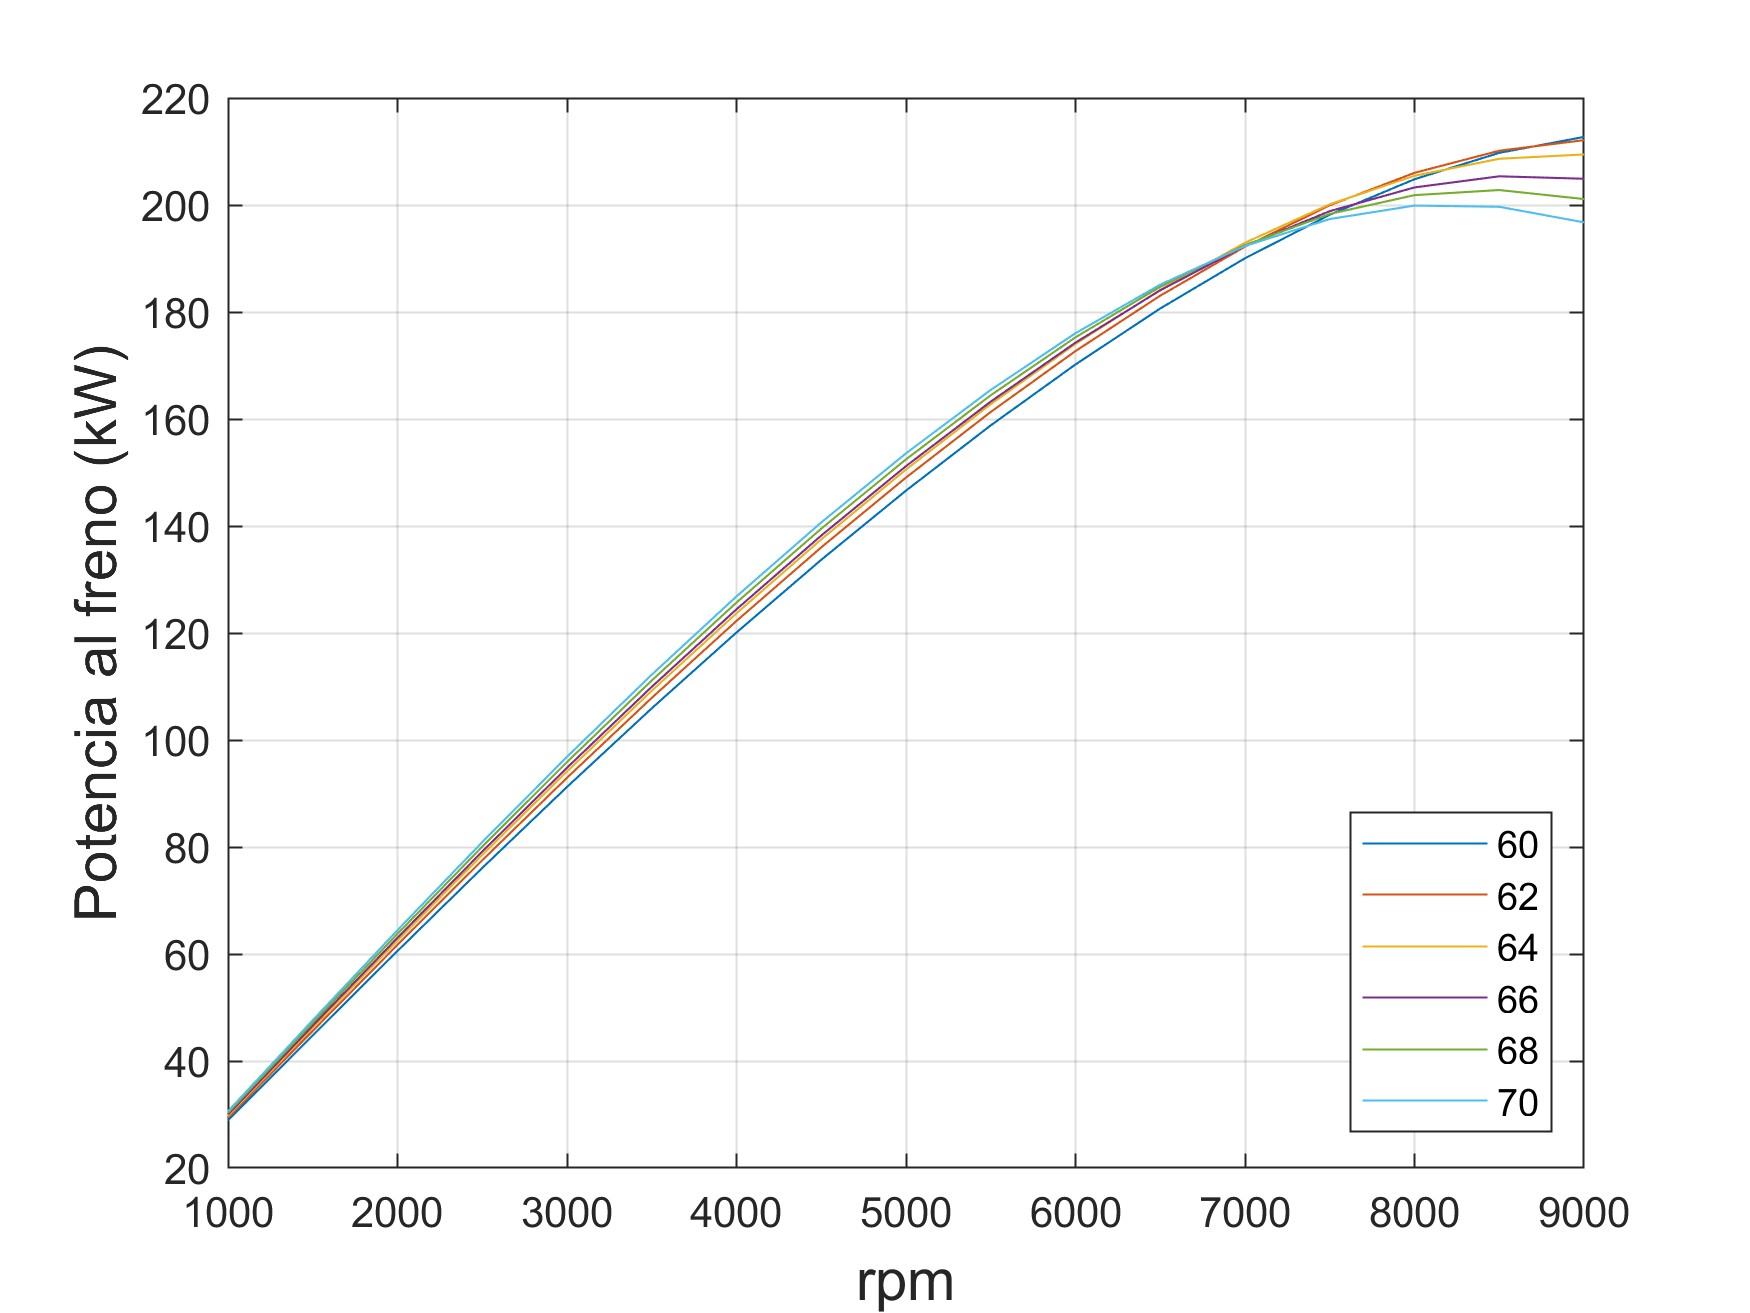
\includegraphics[width=0.6\linewidth]{Figures/01/Potencia_rpm_sb.jpg}
    \caption{Potencia en función de las rpm para cada carrera.}
    \label{fig:RPM_sb}
\end{figure}

La curva de potencia elegida para el estudio se corresponde con una carrera \( s = 62 \, \text{mm} \) y con un radio del émbolo \( b = 101 \, \text{mm} \).

\section{Retardo al Cierre de Admisión} \label{s:section_03}
Para determinar el retardo del cierre de la válvula de admisión se ha ejecutado un bucle que proporciona las curvas de potencia al freno del motor para distintos valores de dicho ángulo. Una vez obtenida esa gráfica (figura \ref{fig:RPM_rca}) se escoge, para cada intervalo de revoluciones, el valor que mayor potencia proporciona. Esos valores se recogen en la tabla \ref{tab:rpm_RCA}, y a partir de ellos se genera un polinomio de orden 3 (implementado a posteriori en una función) de manera que, para un valor arbitrario de revoluciones del motor, se recibe (redondeado al entero más próximo) el valor óptimo de este parámetro. Los resultados de este polinomio y los datos contenidos en la tabla se observan en la figura \ref{fig:RPM_rca_regresión}.

\begin{figure}[H]
    \centering
    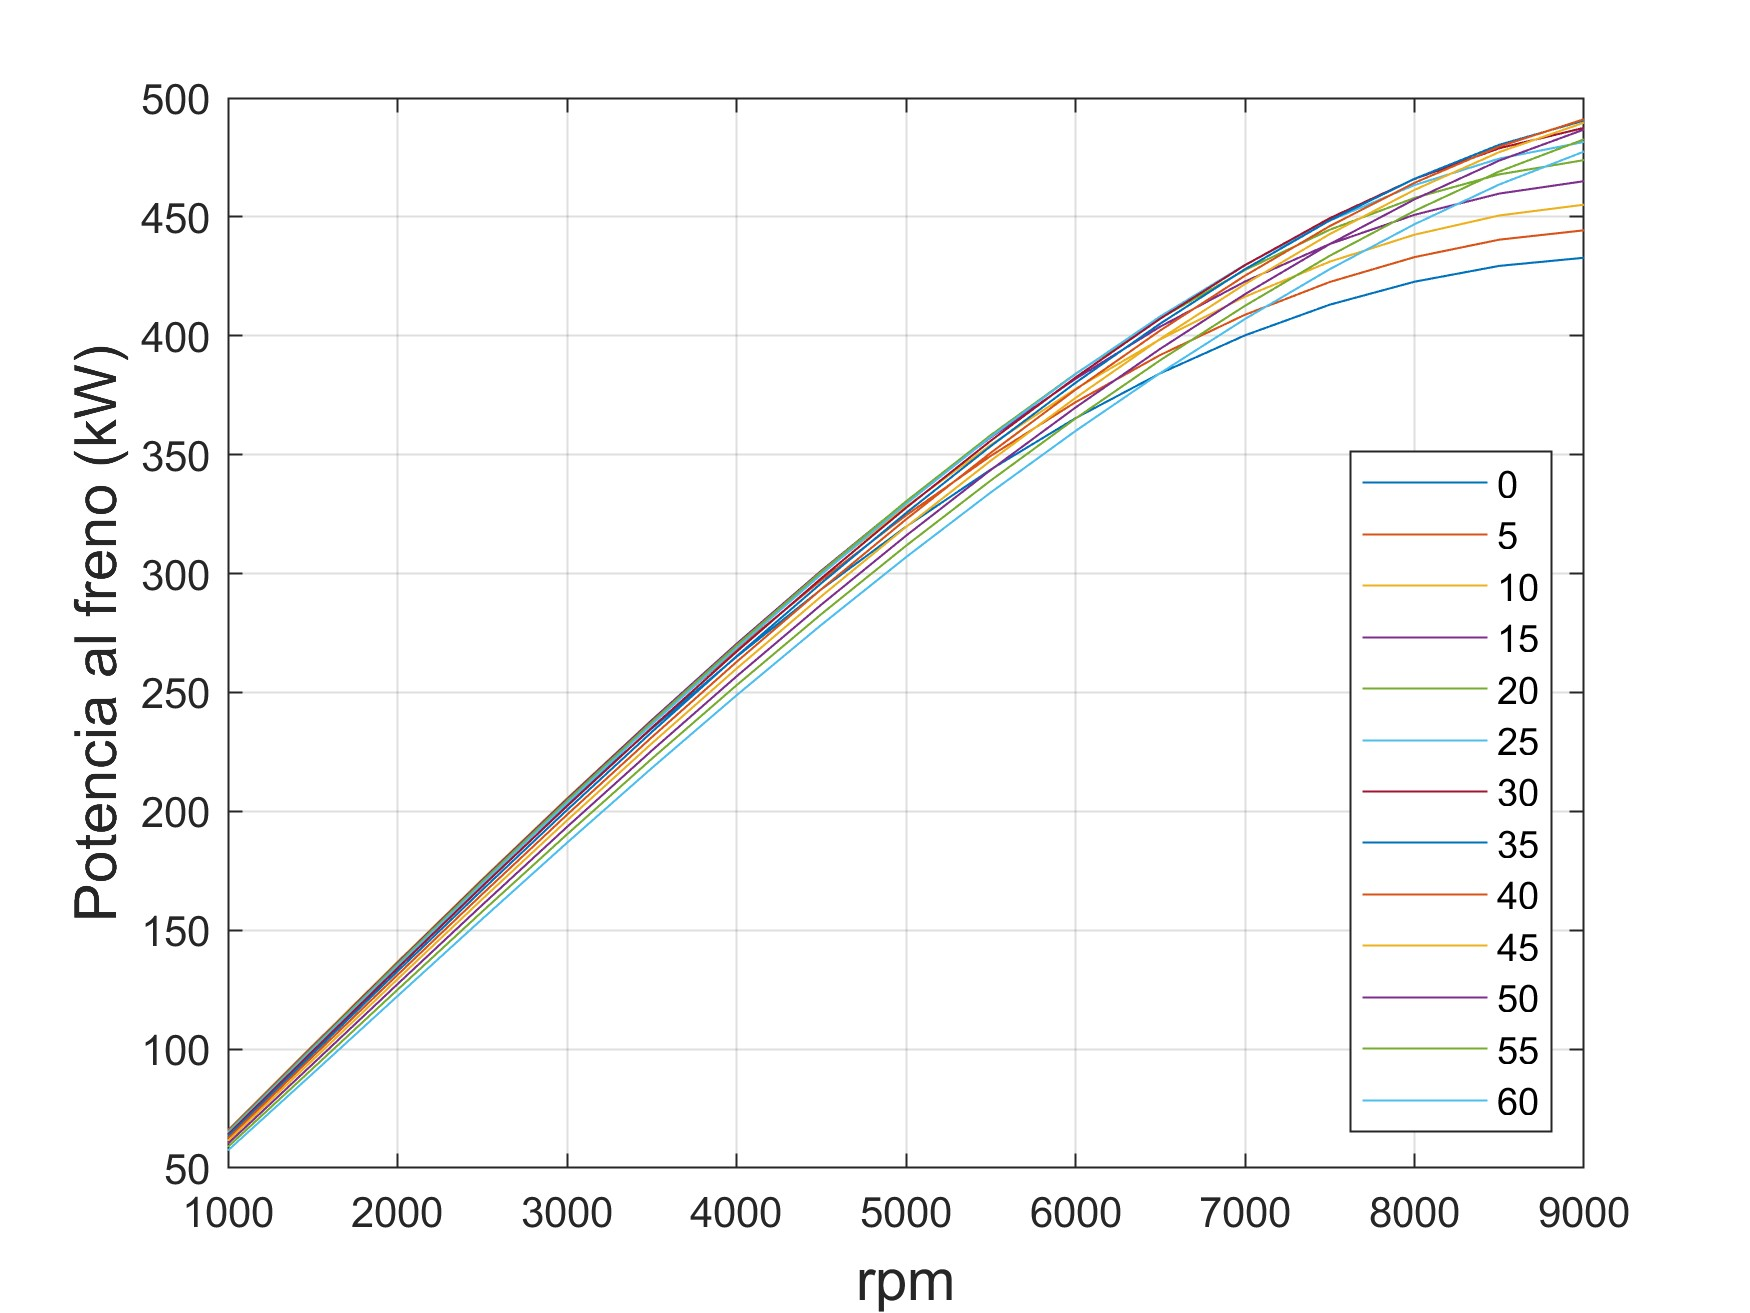
\includegraphics[width=0.6\linewidth]{Figures/01/Potencia_rpm_rca.jpg}
    \caption{Potencia en función de las rpm para cada retardo al cierre de admisión.}
    \label{fig:RPM_rca}
\end{figure}

\begin{table}[htbp]
    \centering
    \resizebox{1\textwidth}{!}{
        \begin{tabular}{|c|*{8}{c|}}
           \hline 
           \textbf{rpm} & 0-2000 & 2000-3500 & 3500-4800 & 4800-6000 & 6000-6900 & 6900-7750 & 7750-8500 & 8500-9000 \\
           \hline 
           RCA [°] & 5 & 10 & 15 & 20 & 30 & 35 & 40 & 45 \\
           \hline
        \end{tabular}
    }
    \caption{Retardos de cierre de admisión que obtienen mayor potencia en función de las rpm.}
    \label{tab:rpm_RCA}
\end{table}

\begin{figure}[H]
    \centering
    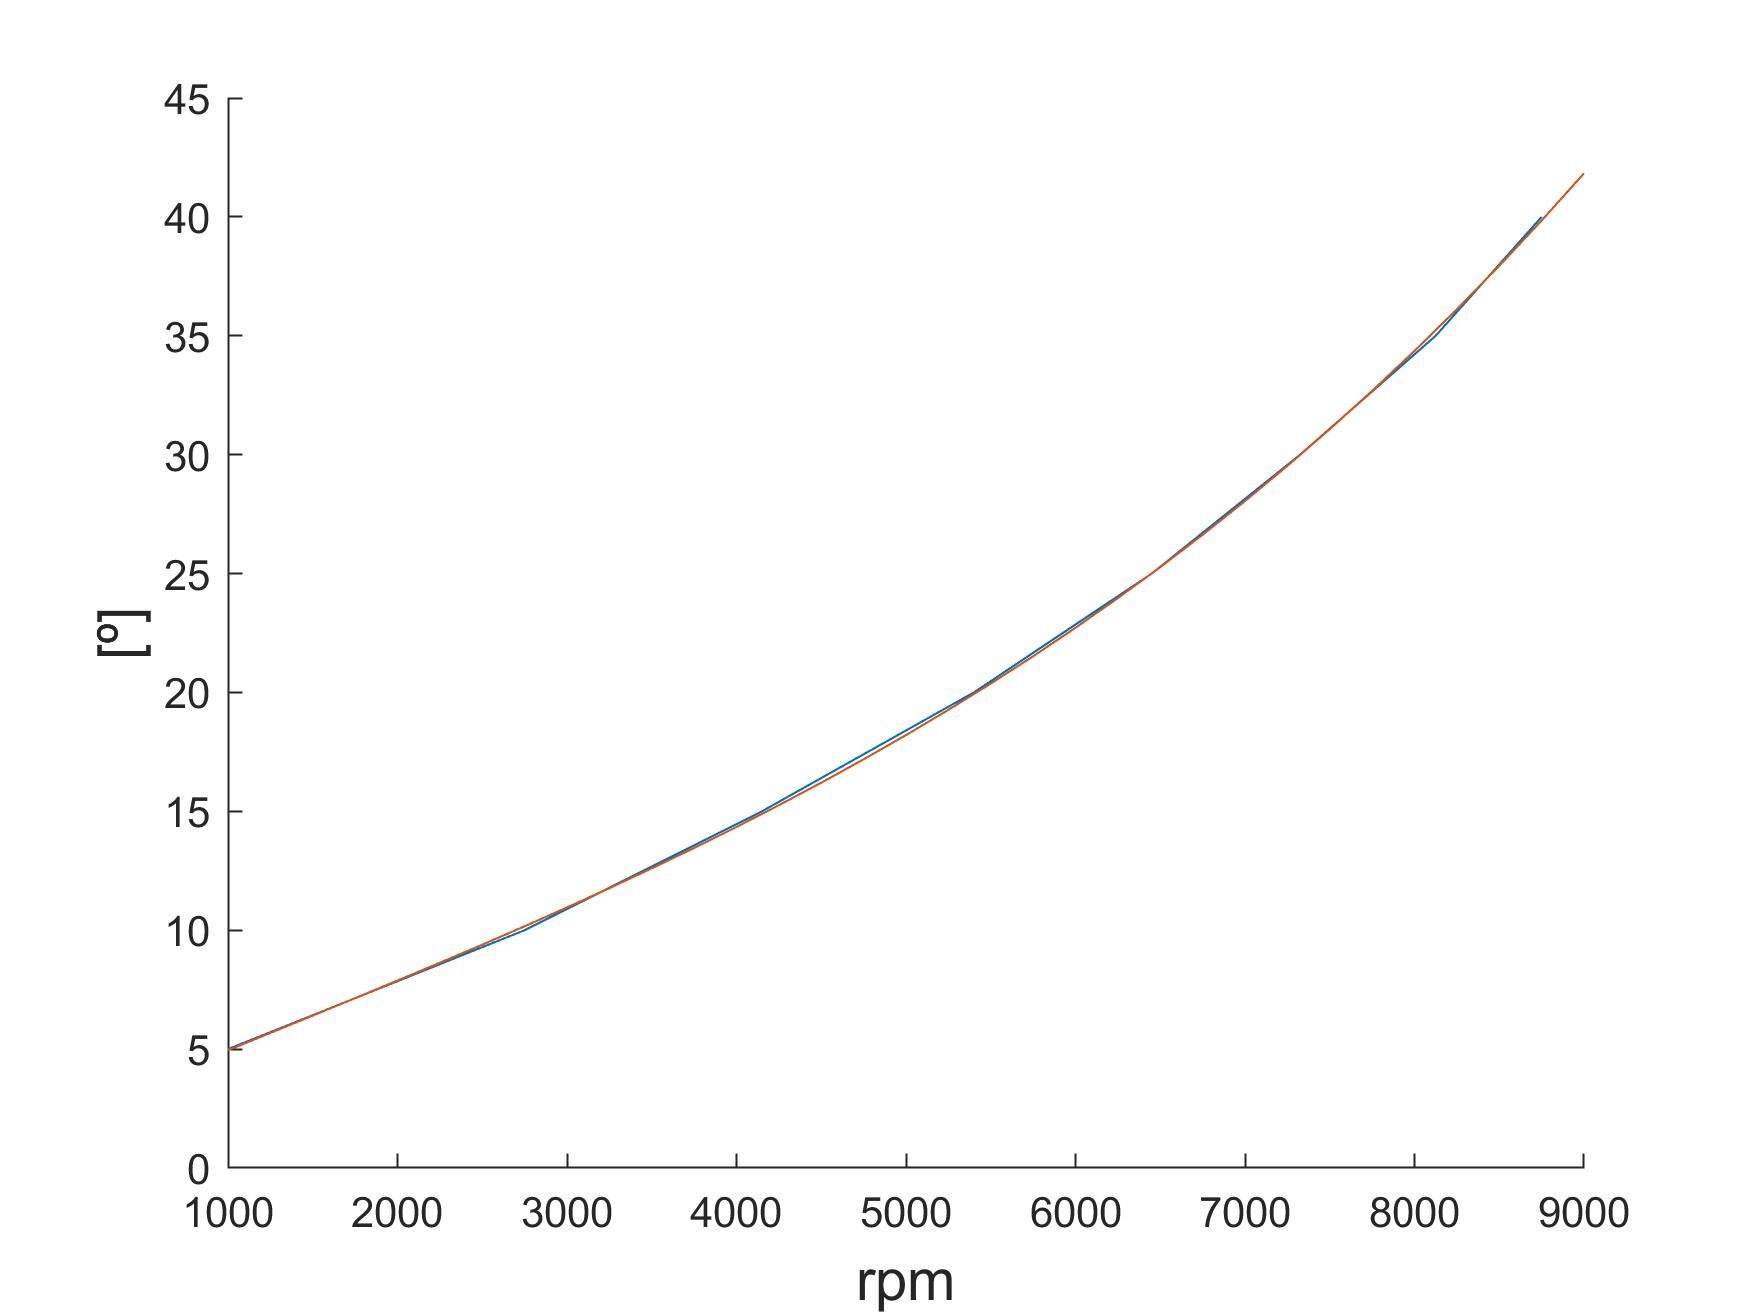
\includegraphics[width=0.6\linewidth]{Figures/01/regresion_rca.jpg}
    \caption{Polinomio del retardo al cierre de admisión en función de las rpm.}
    \label{fig:RPM_rca_regresión}
\end{figure}







\section{Adelanto a la apertura de escape} \label{s:section_04}

Se procede de forma análoga al apartado anterior y se recoge la potencia al freno del motor para distintos valores de dicho ángulo \ref{fig:RPM_aae}. A través de esta gráfica se obtiene la tabla \ref{tab:rpm_AAE}. Los resultados de realizar una regresión igual a la utilizada con el RCA y los datos contenidos en la tabla se observan en la figura \ref{fig:RPM_aae_regresión}.

\begin{figure}[H]
    \centering
    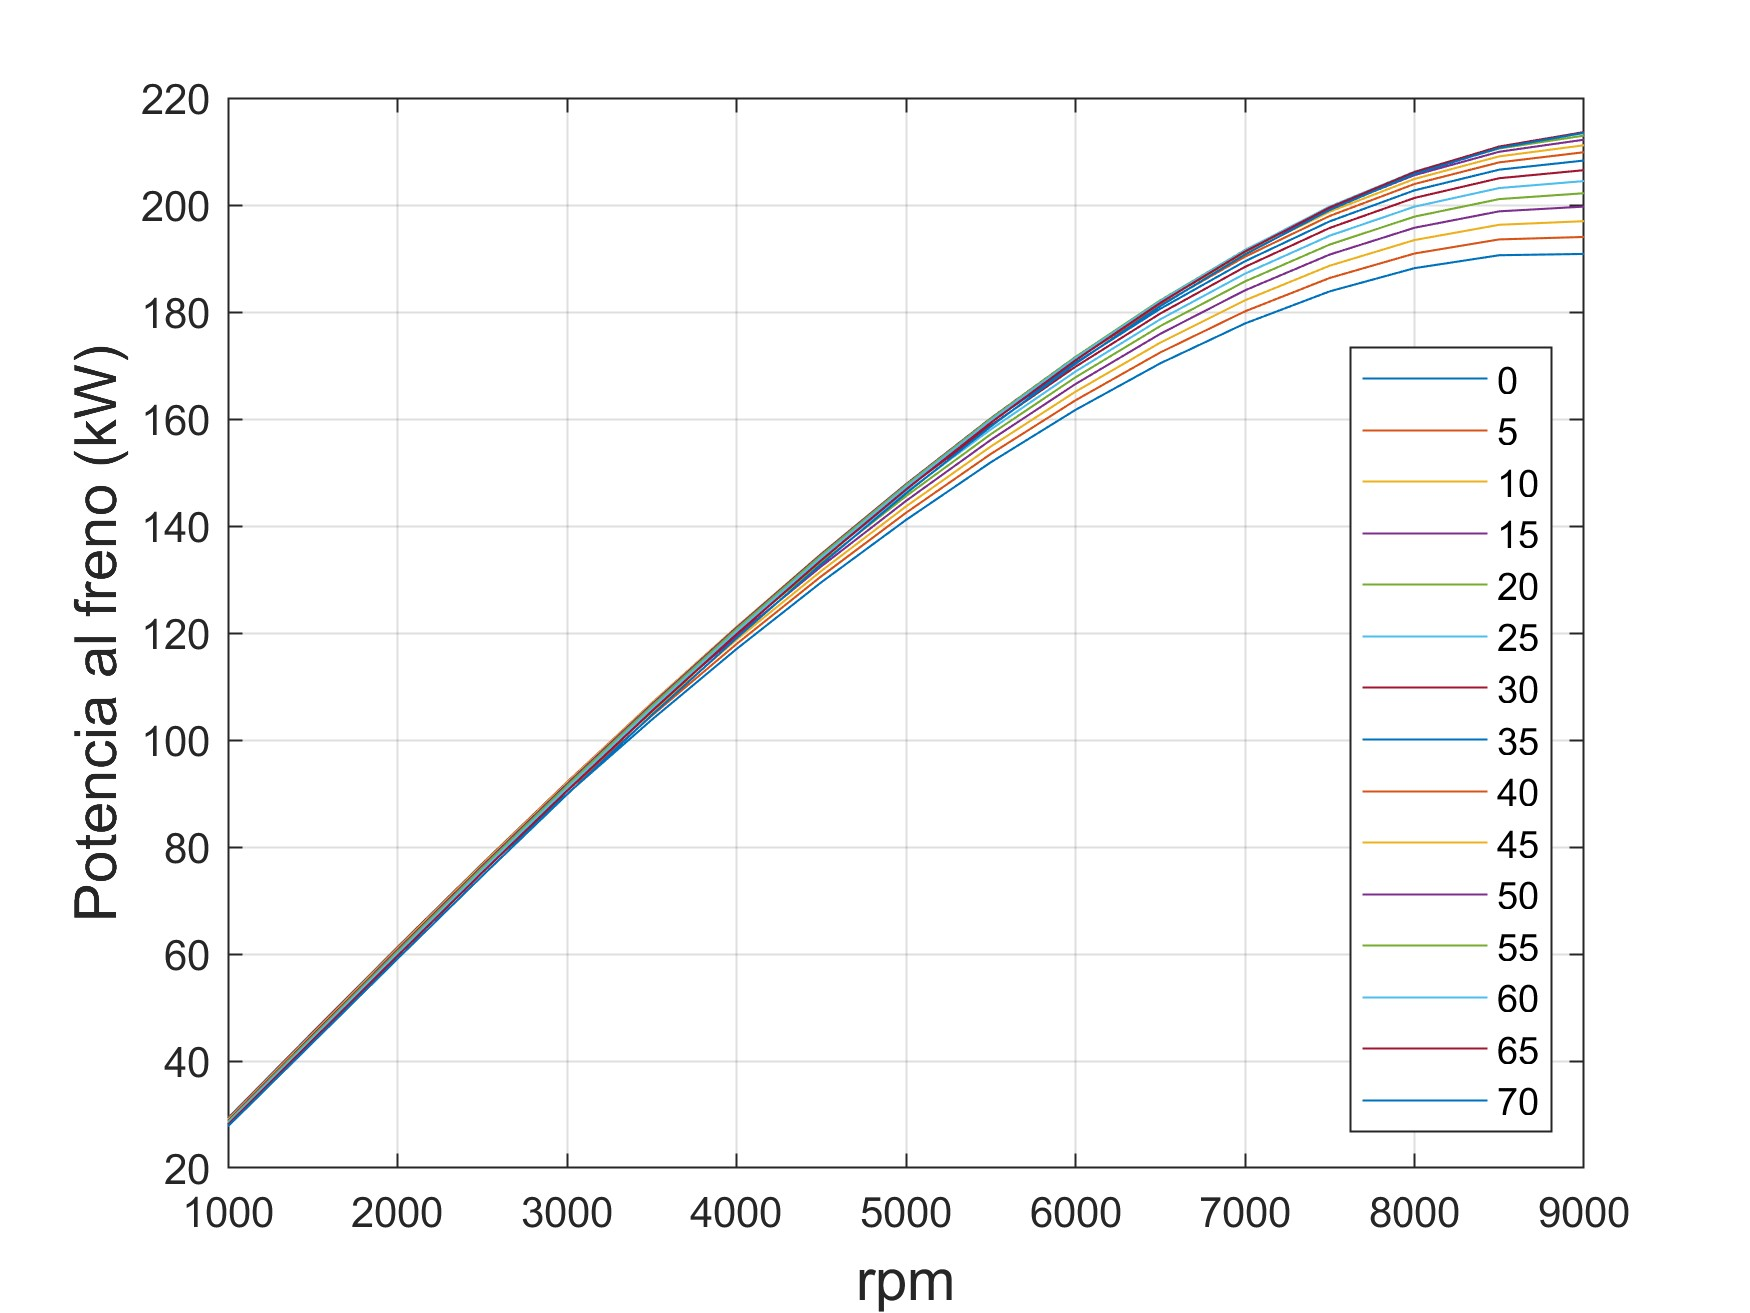
\includegraphics[width=0.6\linewidth]{Figures/01/Potencia_rpm_aae.jpg}
    \caption{Potencia en función de las rpm para cada adelanto a la apertura de escape.}
    \label{fig:RPM_aae}
\end{figure}

\begin{table}[htbp]
    \centering
    \resizebox{1\textwidth}{!}{
        \begin{tabular}{|c|*{9}{c|}}
           \hline 
           \textbf{rpm} & 0-1750 & 1750-2500 & 2500-3250 & 3250-4000 & 4000-5000 & 5000-6000 & 6000-7000 & 7000-8500 & 8500-9000 \\
           \hline 
           RCA [°] & 30 & 35 & 40 & 45 & 50 & 55 & 60 & 60 & 65 \\
           \hline
        \end{tabular}
    }
    \caption{Adelantos de apertura de escape que obtienen mayor potencia en función de las rpm.}
    \label{tab:rpm_AAE}
\end{table}

\begin{figure}[H]
    \centering
    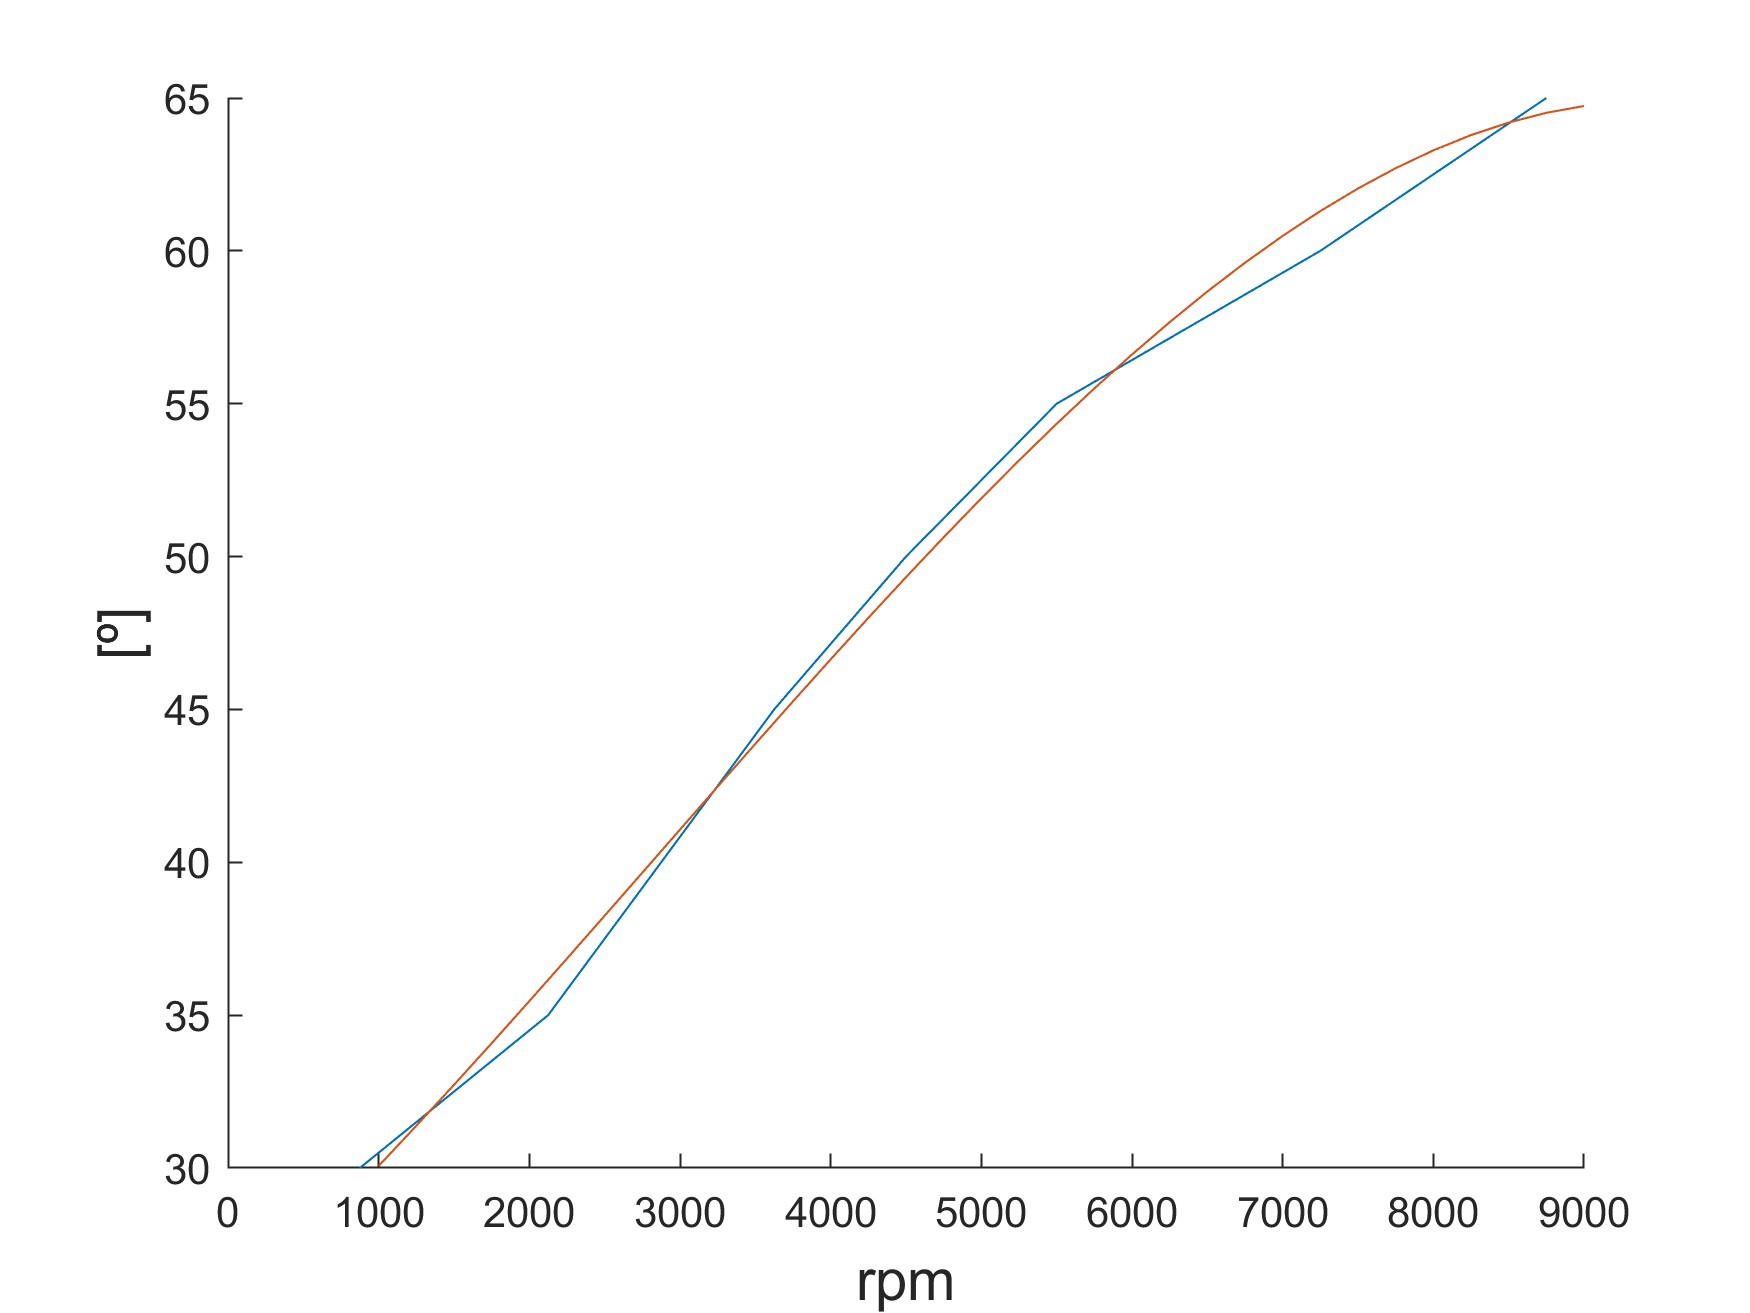
\includegraphics[width=0.6\linewidth]{Figures/01/regresion_aae.jpg}
    \caption{Polinomio del adelanto de apertura de escape en función de las rpm.}
    \label{fig:RPM_aae_regresión}
\end{figure}



\section{Elección de los Parámetros} \label{s:section_05}
\subsection{Relación de Compresión Geométrica} \label{s:subsection_01}
Inicialmente se empleó una relación de compresión de 7.5, al ver que este se podía subir sin generar problemas de detonación que no se pudiesen solucionar modificando los ángulos de ignición, se decidió subir a 9.5. A su vez, al haber elegido un vehículo deportivo turboalimentado, en la modelización de este se considera una presión de admisión algo mayor que la correspondiente con la ambiente al nivel del mar; es decir, alrededor de 2 bares; mientras que la presión de escape será el 80\% de esta última.

\subsection{Áreas de válvulas} \label{s:subsection_02}
\begin{itemize}
   \item \textbf{Área de válvula de admisión (AA):} 33\%  del área del cilindro.
  \item \textbf{Área de válvula de escape (AE):} 28\%  del área del cilindro.
  \end{itemize}

A partir de esta configuración inicial, se evalúa el impacto de variaciones, en este caso, aumento; en el tamaño del área efectiva de las válvulas sobre el rendimiento del motor.

\begin{figure}[H]
    \centering
    \begin{subfigure}[b]{0.45\textwidth}
        \centering
        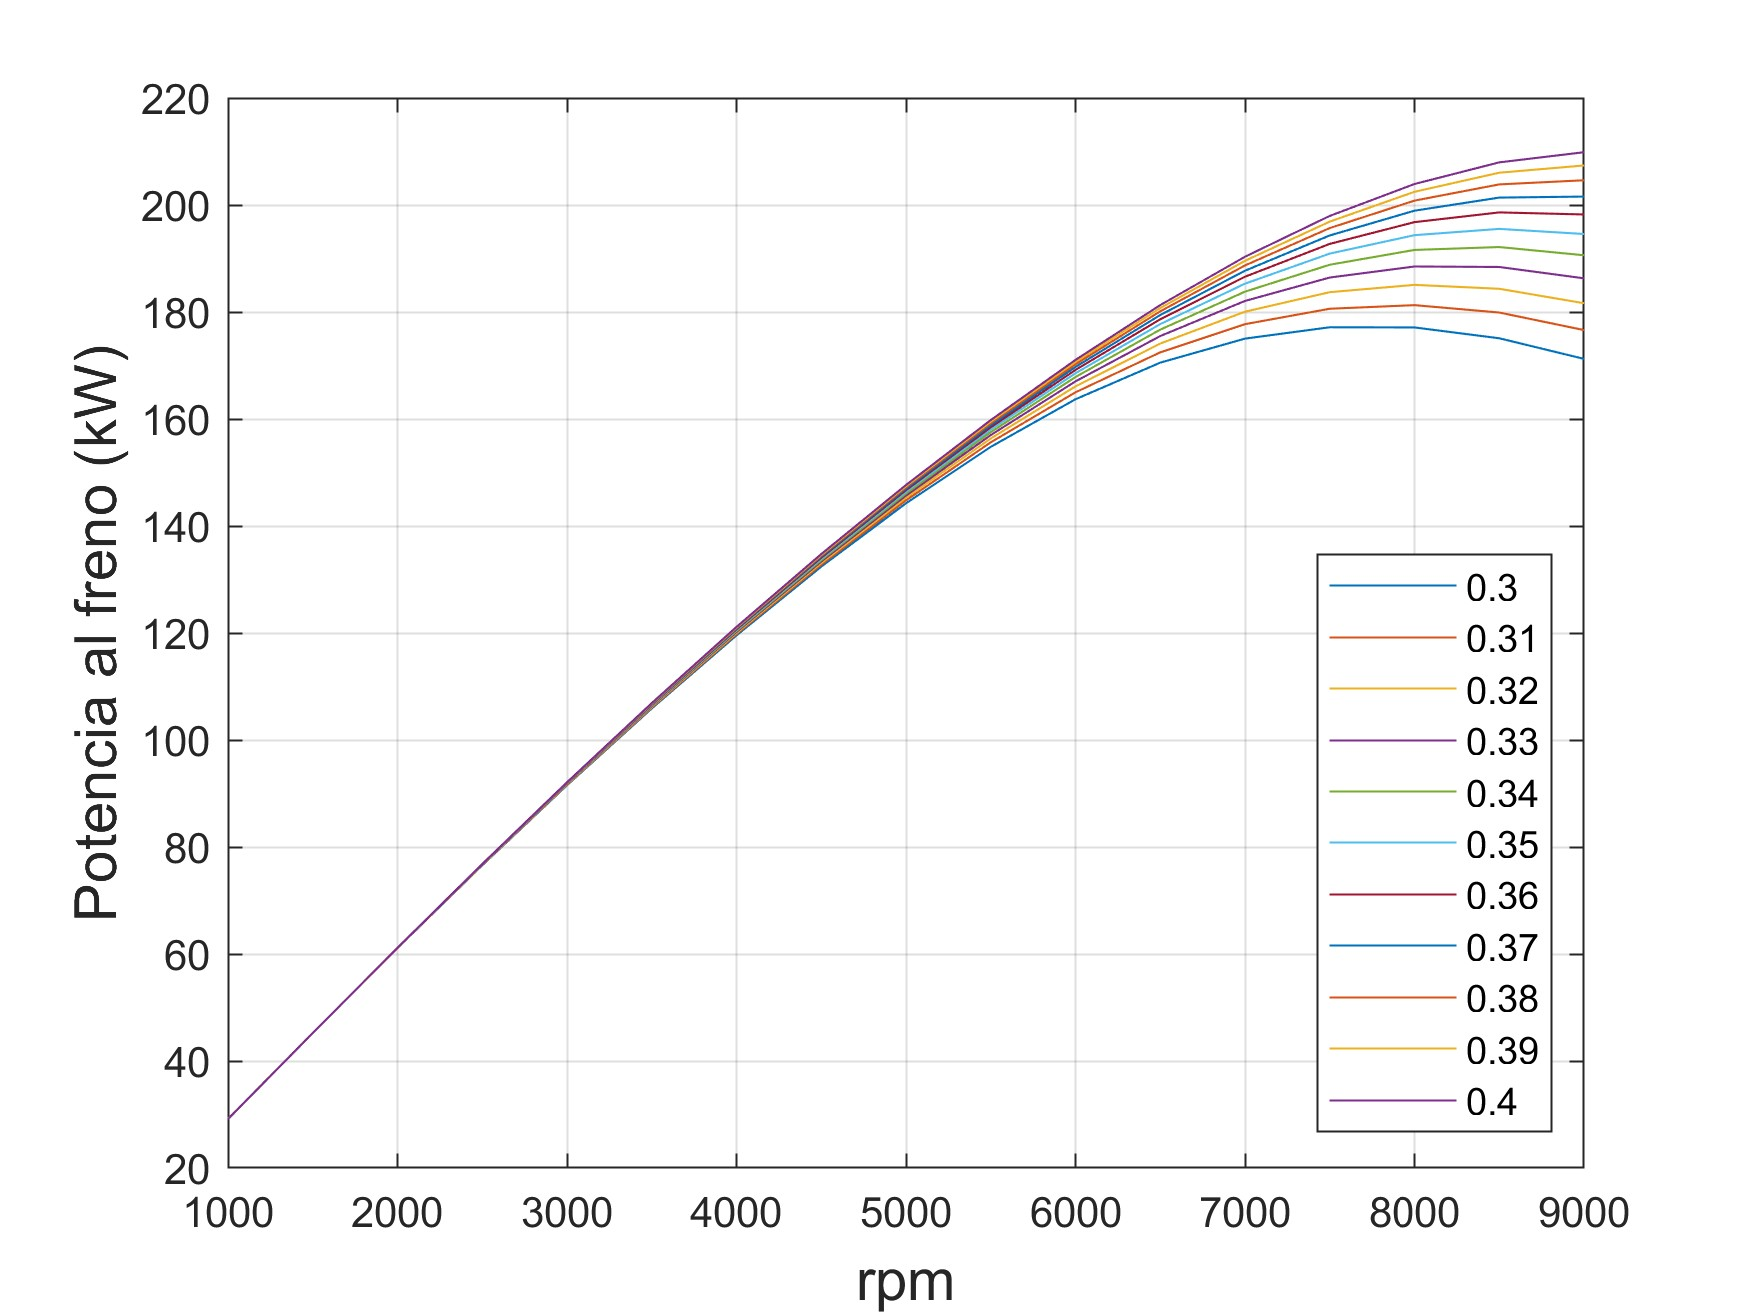
\includegraphics[width=\linewidth]{Figures/01/Potencia_rpm_aval_admision.jpg}
        \caption{Potencia en función de las rpm para dicha área de válvula de admisión (AA).}
        \label{fig:RPM_aval_admision}
    \end{subfigure}
    \hfill
    \begin{subfigure}[b]{0.45\textwidth}
        \centering
        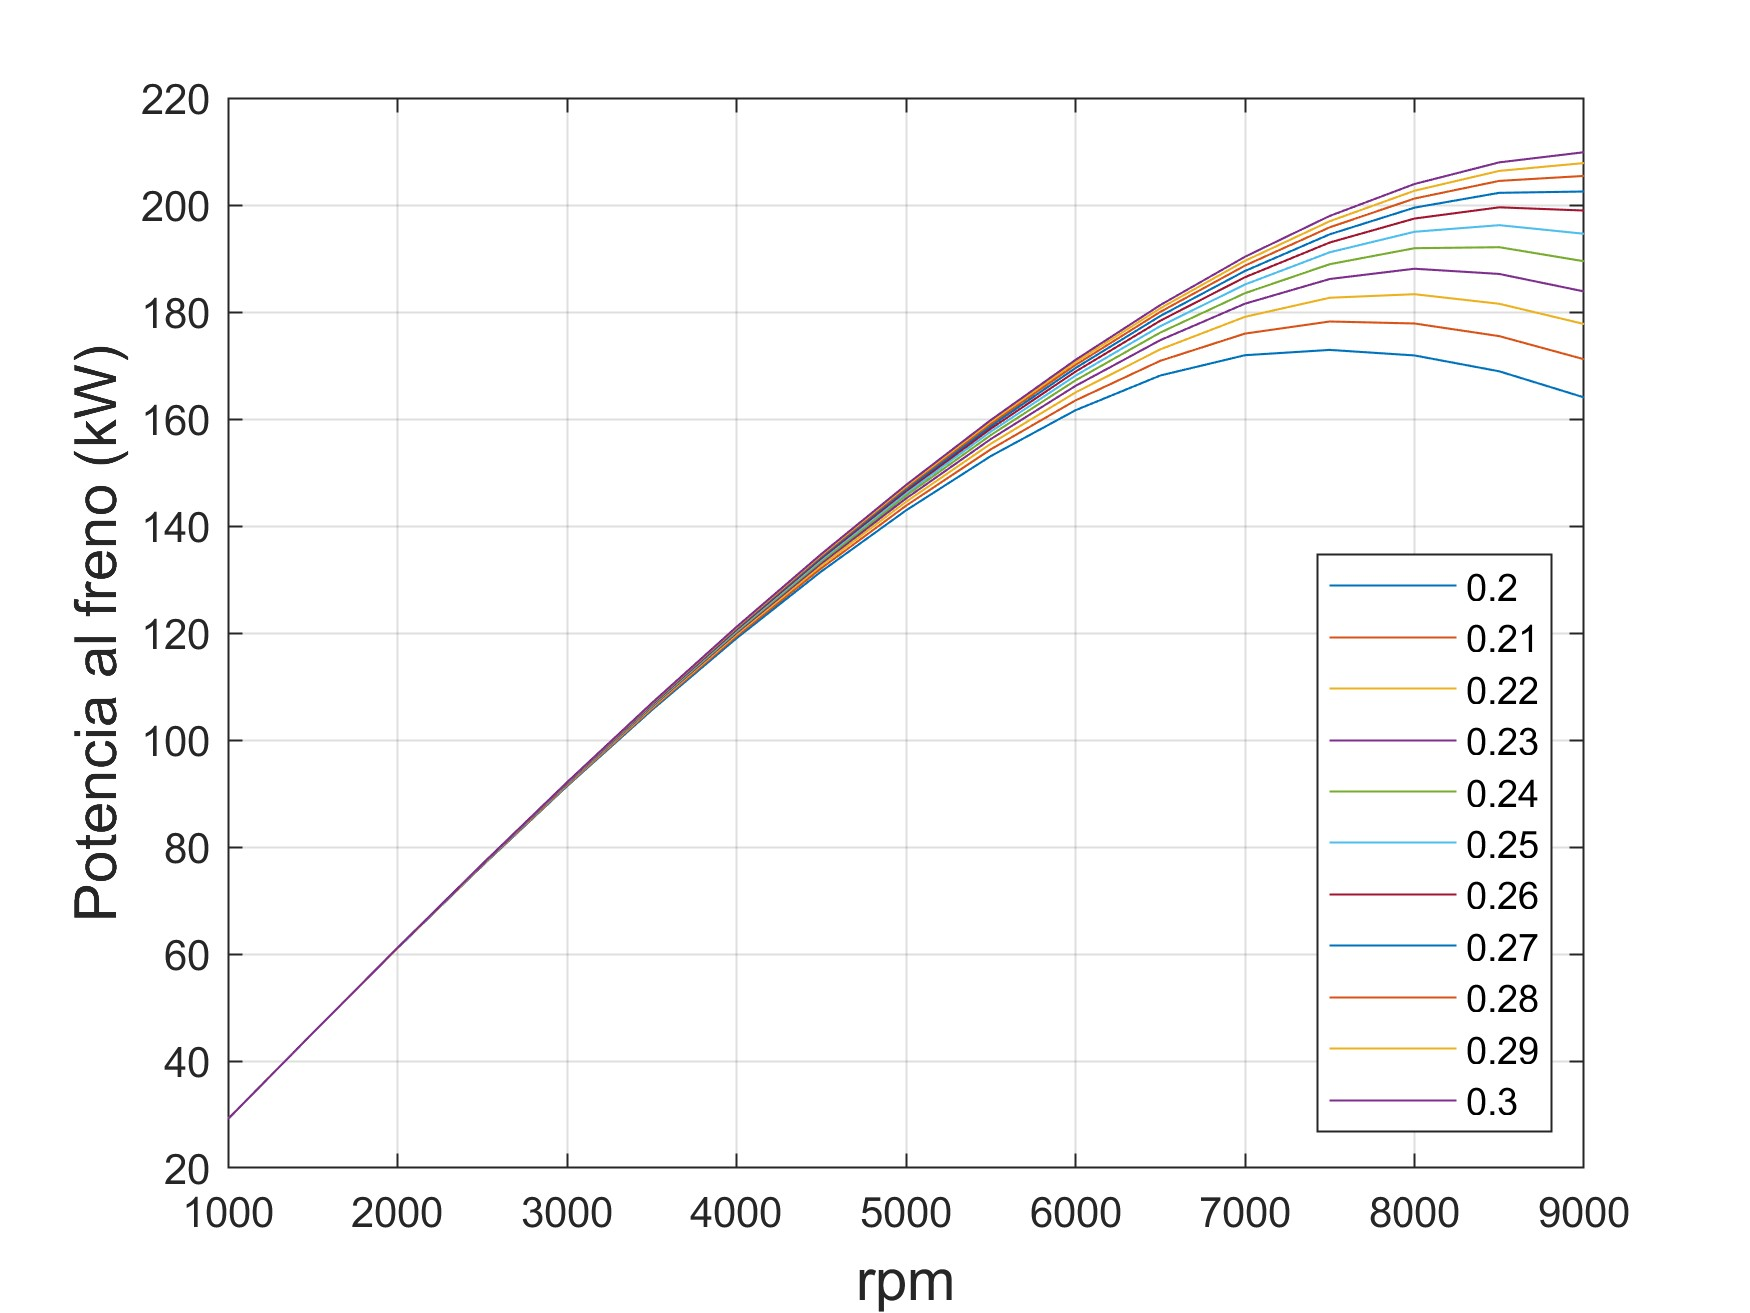
\includegraphics[width=\linewidth]{Figures/01/Potencia_rpm_aval_escape.jpg}
        \caption{Potencia en función de las rpm para dicha área de válvula de escape (AE).}
        \label{fig:RPM_aval_escape}
    \end{subfigure}
    
    \caption{Potencia en función de las rpm para áreas de válvula de admisión (AA) y de escape (AE).}
    \label{fig:RPM_aval_combined}
\end{figure}

Como era de esperar, se comprueba que un aumento en el tamaño de las válvulas implica un aumento en el flujo de aire que entra al motor y, por tanto, en la potencia producida por el mismo. Sin embargo, existe una limitación geométrica y de propiedades del material a la hora de ir aumentando el tamaño de los agujeros practicados a la culata para alojar dichas válvulas. Por tanto, se tomaron los siguientes valores:

\begin{itemize}
   \item \textbf{Área de válvula de admisión (AA):} 40\%  del área del cilindro.
  \item \textbf{Área de válvula de escape (AE):} 30\%  del área del cilindro.
  \end{itemize}
  

\subsection{Curva de Avance de Encendido} \label{s:subsection_03}

Para determinar la curva de avance de encendido a plena carga del motor se ejecutó un bucle de código que recorre los puntos de funcionamiento a plena carga (presión de soplado del turbo 2.1 bar), con un paso de $50 \ rpm$, y un barrido desde $-20º$ a $40º$ de adelanto de encendido frente al punto muerto superior del tiempo de compresión (siendo valores negativos de AICB retardos), mientras que se guarda en un vector el peligro de detonación para cada una de las combinaciones. Se escoge, entonces, para cada valor de $rpm$, el valor de AICB que más próximo se quede, por debajo, a un peligro de detonación de $1.05$. Mediante esos datos se genera un polinomio de grado 6 que aproxime a la función discreta. Dicho polinomio es la curva analítica que se utiliza para calcular el avance de encendido óptimo a cada régimen de revoluciones.

En la siguiente tabla \ref{tab:rpm_AICB} se presentan algunos de los adelantos de inicio de combustión que evitan la detonación.
\begin{table}[htbp]
    \centering
    \begin{tabular}{|c|c|c|c|c|c|c|c|c|c|}
        \hline
        \textbf{rpm}       & 1000 & 1500 & 2000 & 2500 & 3000 & 3500 & 4000 & 4500 & 5000 \\ 
        \hline
        \textbf{AICB [º]} & -16  & -8   & -2   & 2    & 4    & 6    & 8    & 10   & 10   \\ 
        \hline
        \textbf{rpm}       & 5500 & 6000 & 6500 & 7000 & 7500 & 8000 & 8500 & 9000 & \\ 
        \hline
        \textbf{AICB [º]} & 12   & 14   & 14   & 14   & 16   & 16   & 18   & 18    & \\ 
        \hline
    \end{tabular}
    \caption{Adelantos de inicio de combustión que evitan la detonación en función de las rpm.}
    \label{tab:rpm_AICB}
\end{table}

\begin{figure}[H]
    \centering
    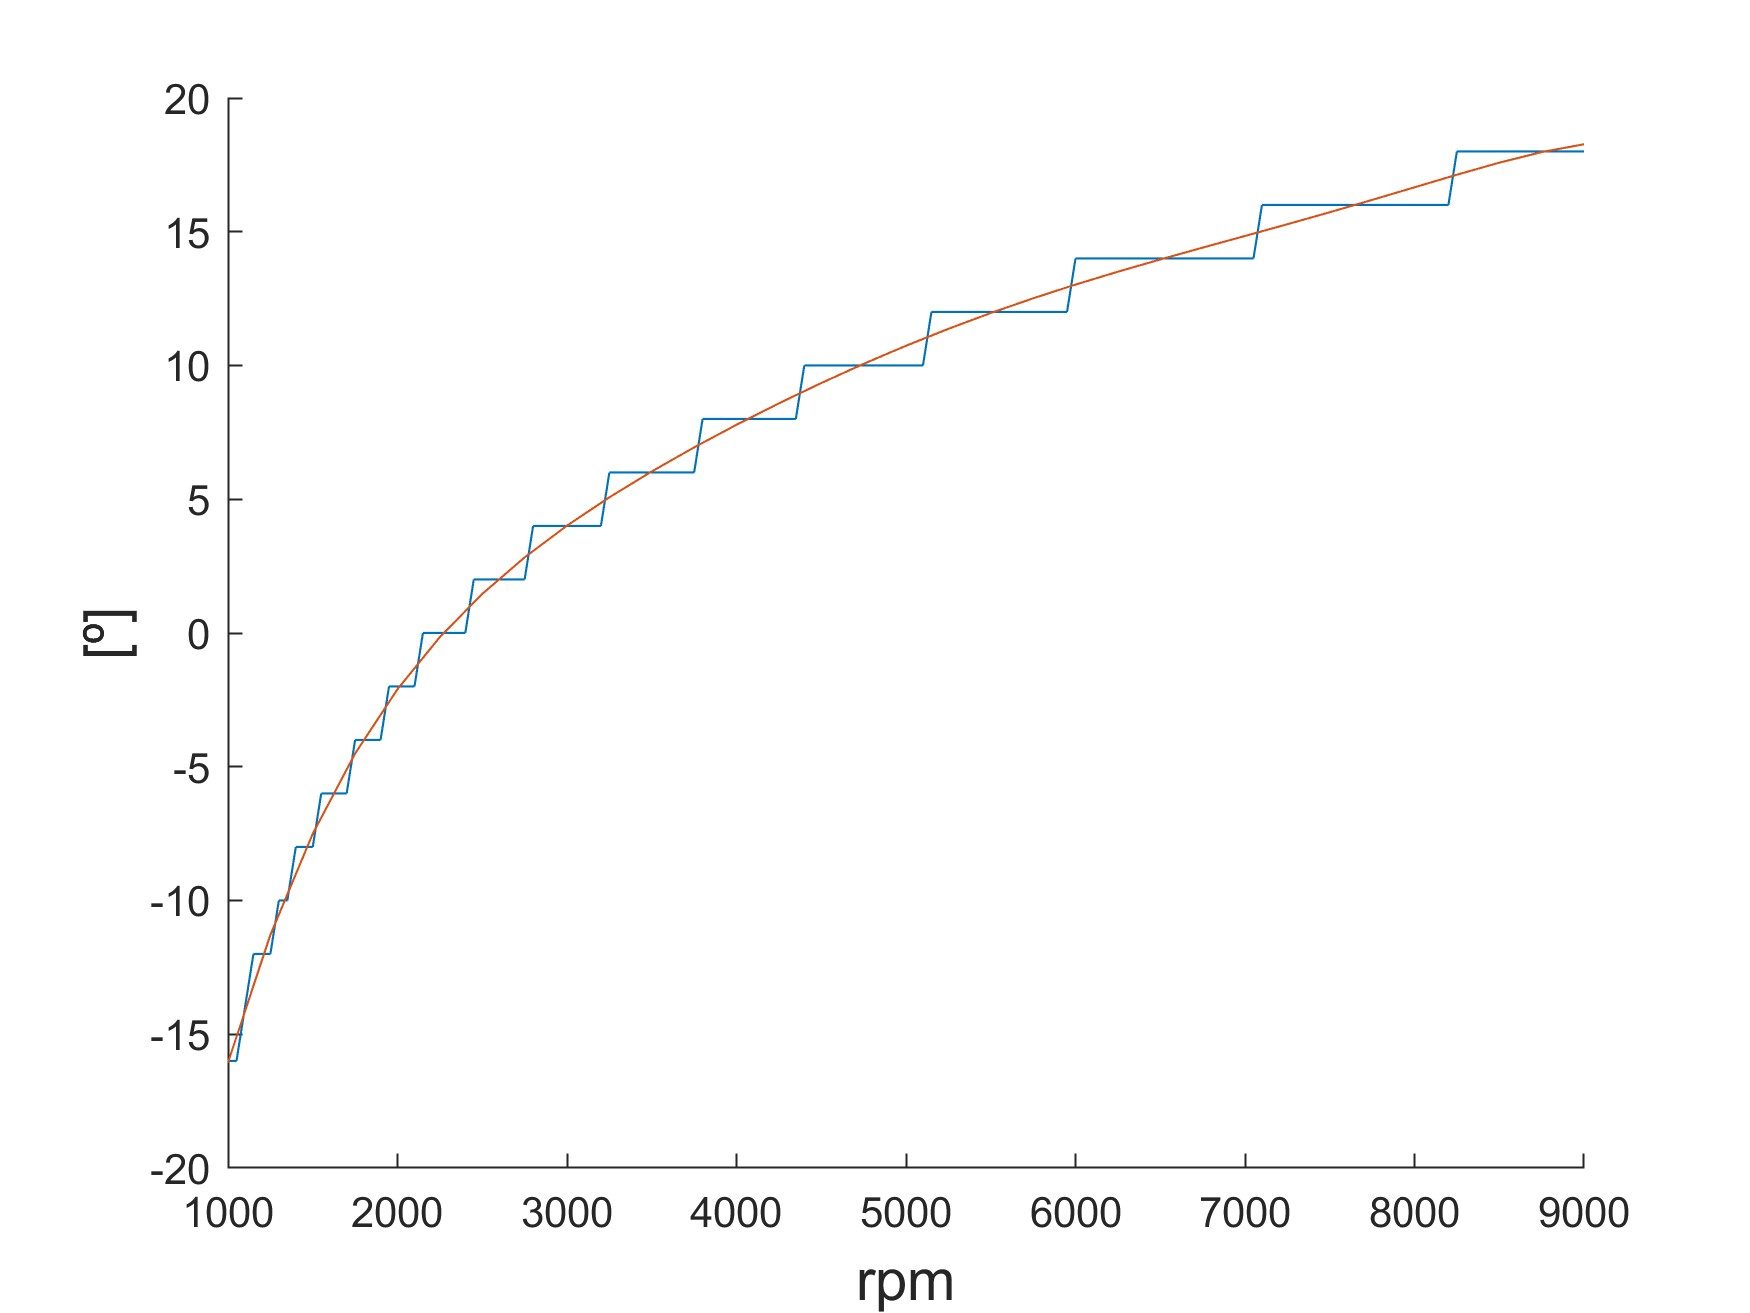
\includegraphics[width=0.6\linewidth]{Figures/01/regresion_aicb.jpg}
    \caption{Adelantos de inicio de combustión que evitan la detonación en función de las rpm.}
    \label{fig:RPM_aicb}
\end{figure}

\section{Actuaciones del motor} \label{s:section_06}

A continuación se presentan las gráficas de par y potencia frente a \textit{rpm}, de consumo específico (BSFC) y de presión media efectiva al freno (BMEP) del motor finalizado. Cabe destacar que las gráficas de BMEP y BSFC siguen comportamientos similares entre sí, teniendo sus extremos en regímenes similares. Además, por conocimiento de los autores, se puede comentar que al ser un motor turboalimentado, se esperaría un pico en las curvas de BMEP y potencia en el momento en el que el turbocompresor comenzase entregar la presión superior a la ambiente (a bajo régimen es complicado, pues los gases de escape no tienen la suficiente potencia para suministrar a la turbina y que esta mueva el compresor).

\begin{figure}[H]
	\centering
	\begin{subfigure}[b]{0.45\textwidth}
   		 \centering
		 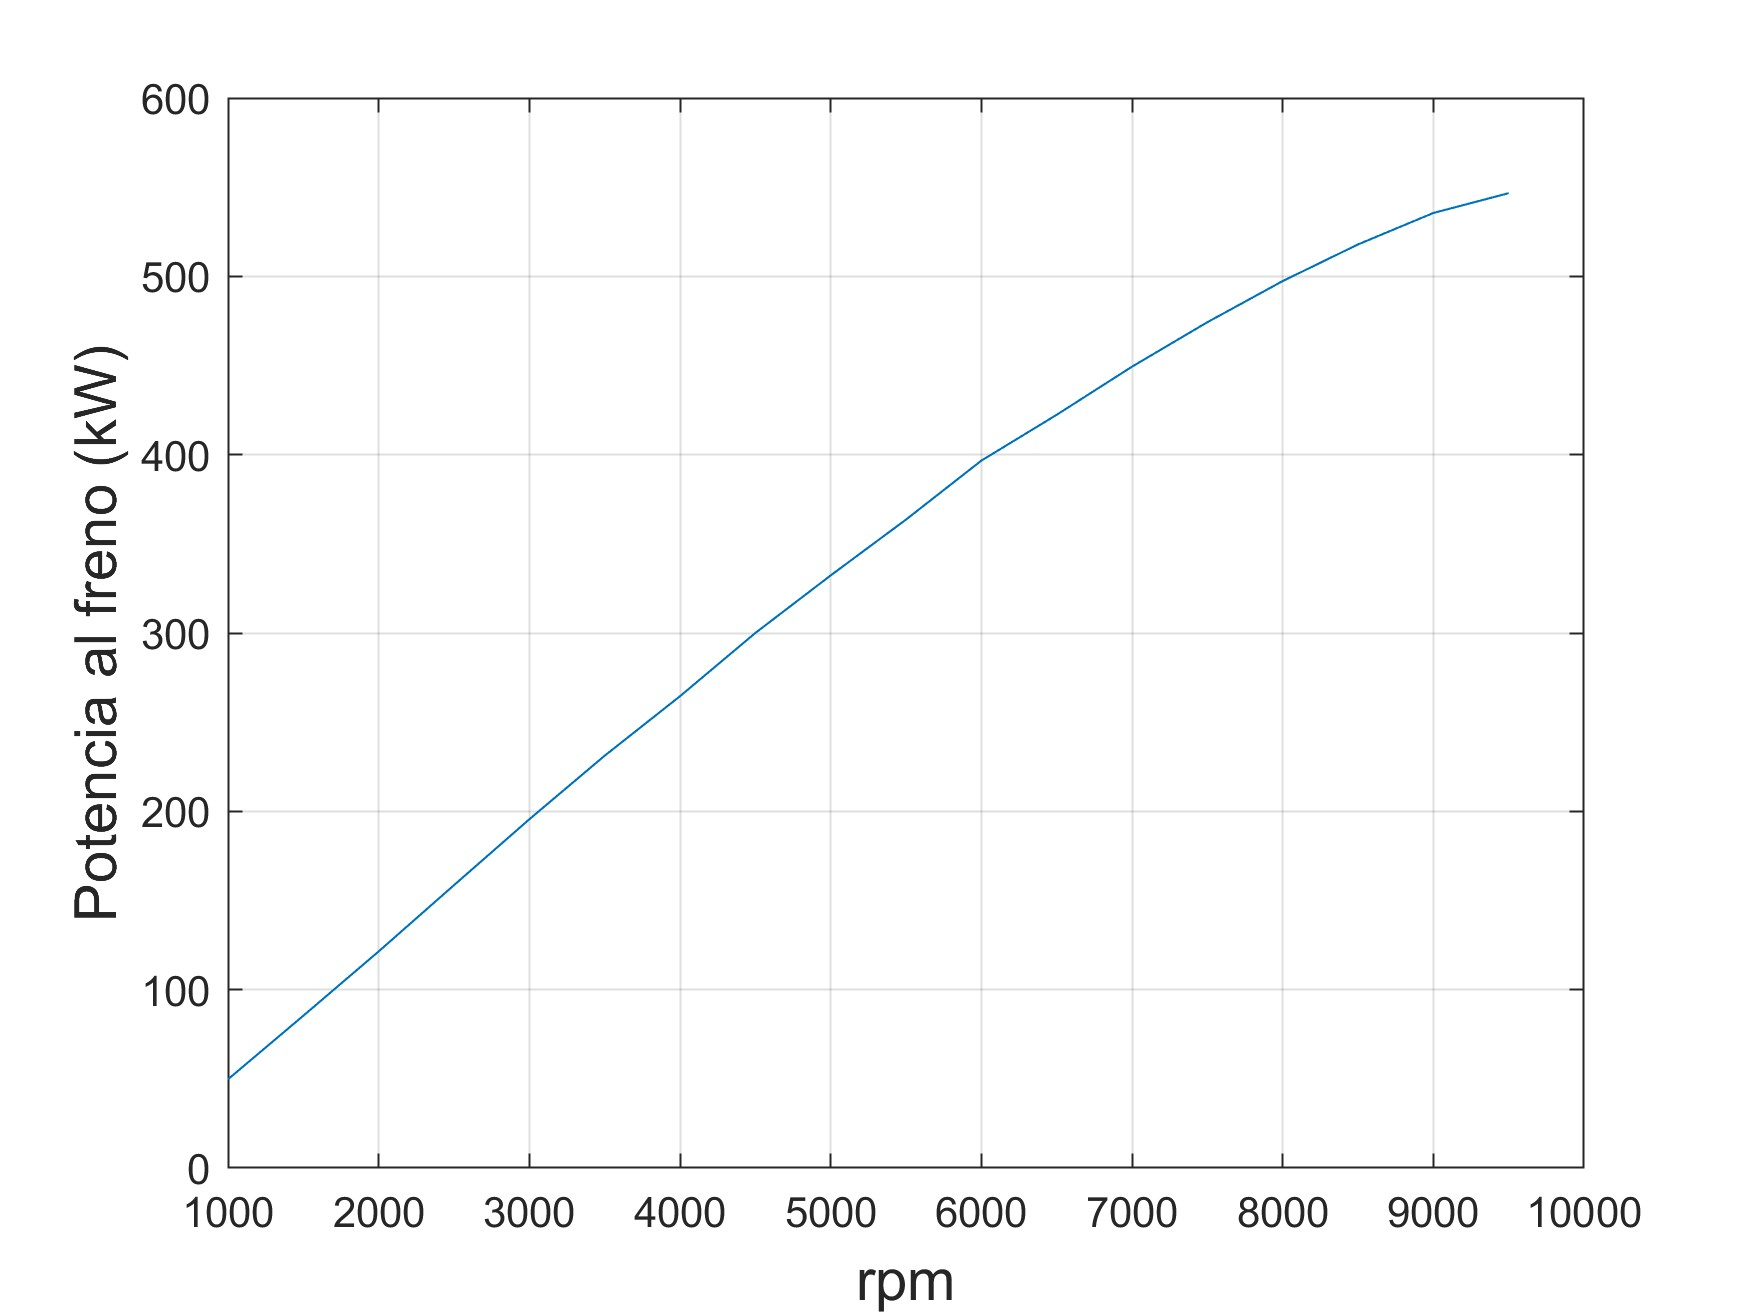
\includegraphics[width=\linewidth]{Figures/01/Potencia_rpm.jpg}
		 \caption{Potencia y par al freno.}
	\end{subfigure}
	\hfill
	\begin{subfigure}[b]{0.45\textwidth}
   		 \centering
		 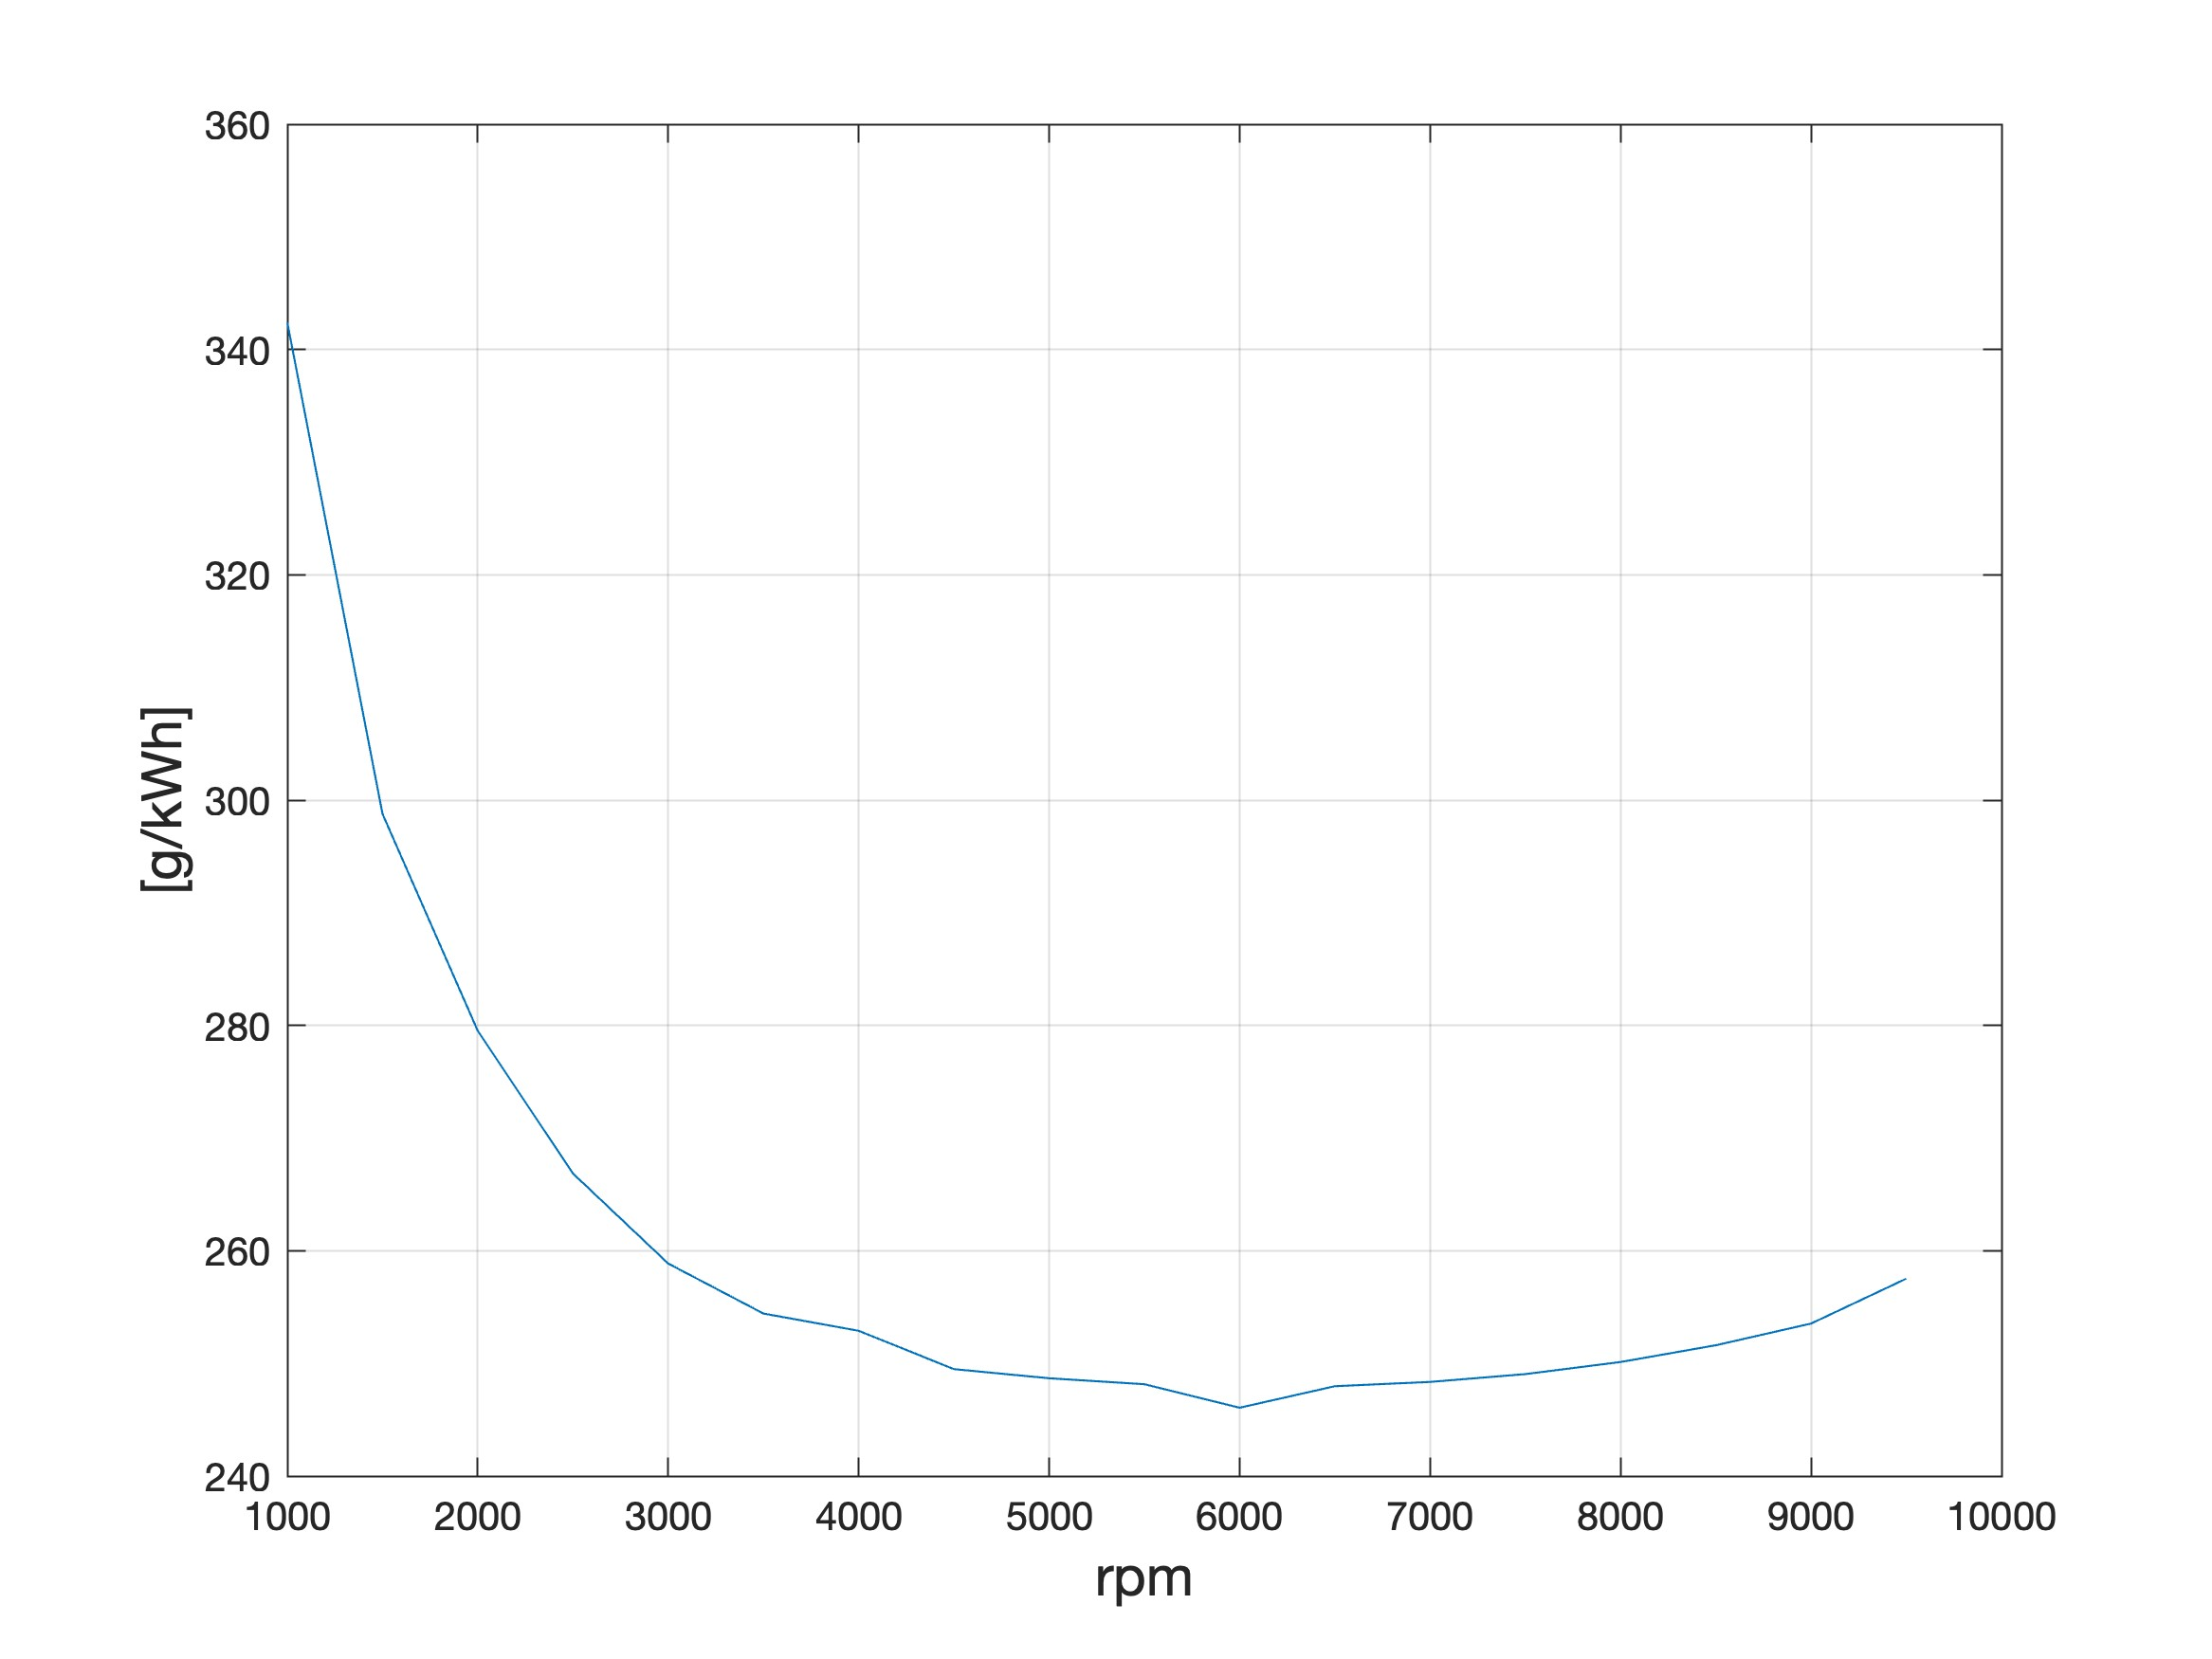
\includegraphics[width=\linewidth]{Figures/01/BSFC_rpm.jpg}
		 \caption{Consumo específico.}
	\end{subfigure}
	
	\caption{Potencia, par y consumo específico en función de las revoluciones.}
	\label{fig:RPM_power}
\end{figure}

\begin{figure}[H]
    \centering
    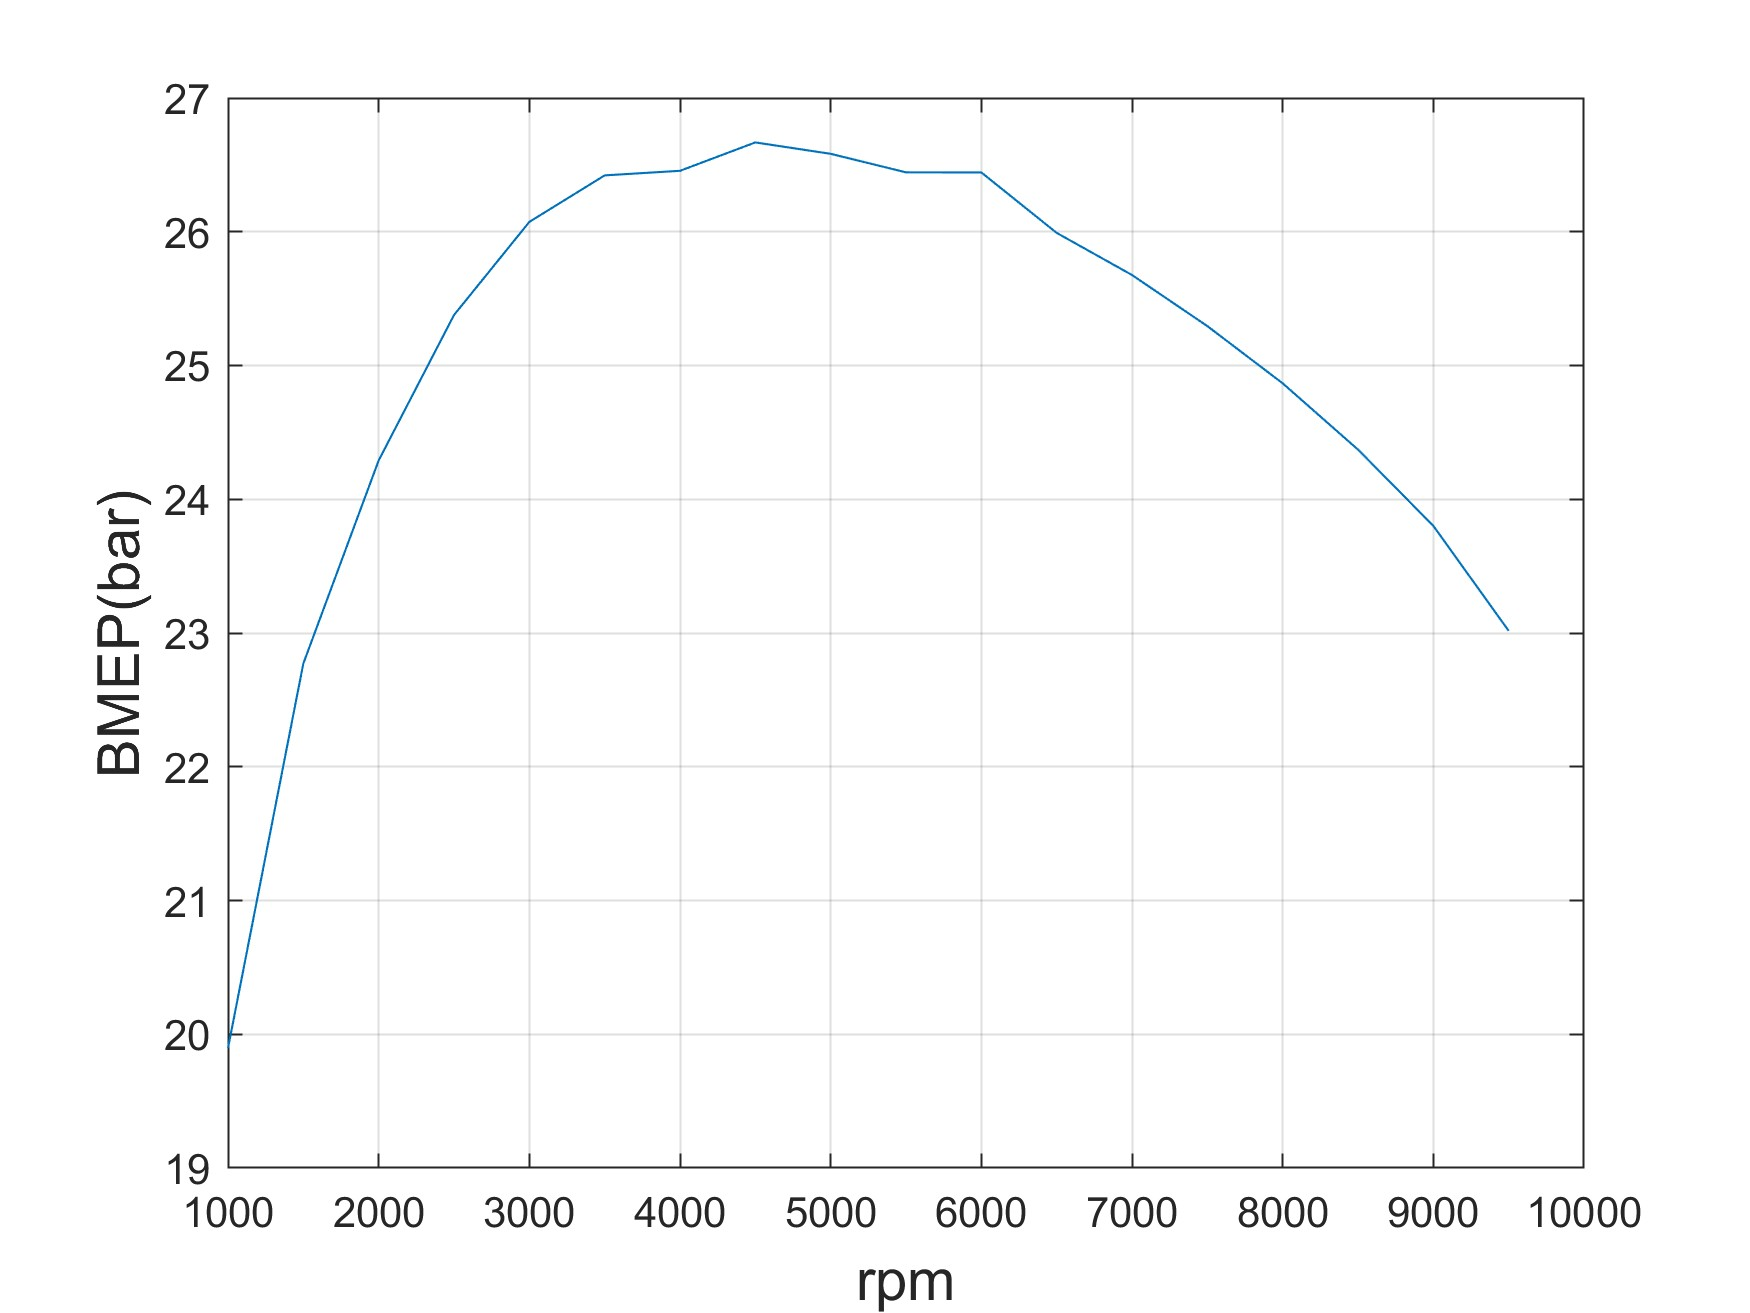
\includegraphics[width=0.6\linewidth]{Figures/01/BMEP.jpg}
    \caption{Presión media efectiva al freno en función de las rpm.}
    \label{fig:RPM_bmep}
\end{figure}

\section{Mapa de encendido} \label{s:section_07}

Se ha desarrollado, de igual manera que se explicó en la sección \ref{s:subsection_03}, el mapa de encendido para todos los regímenes de funcionamiento del motor, iterando esta vez también en las presiones de admisión, desde $0.4\ bar$ hasta $2.1\ bar$, y escogiendo el avance de encendido de una manera idéntica a la antes explicada. El mapa obtenido queda reflejado en la figura \ref{fig:mapa_completo}. Se observa para regímenes de bajas revoluciones y presiones de admisión una  "meseta" , dicha meseta se corresponde a que para esas revoluciones no se está demandando potencia del motor, por lo que no es necesario (ni beneficioso), adelantar el encendido, con el peligro que ello conlleva de que se produzca detonación en el motor.

\begin{figure}[H]
    \centering
    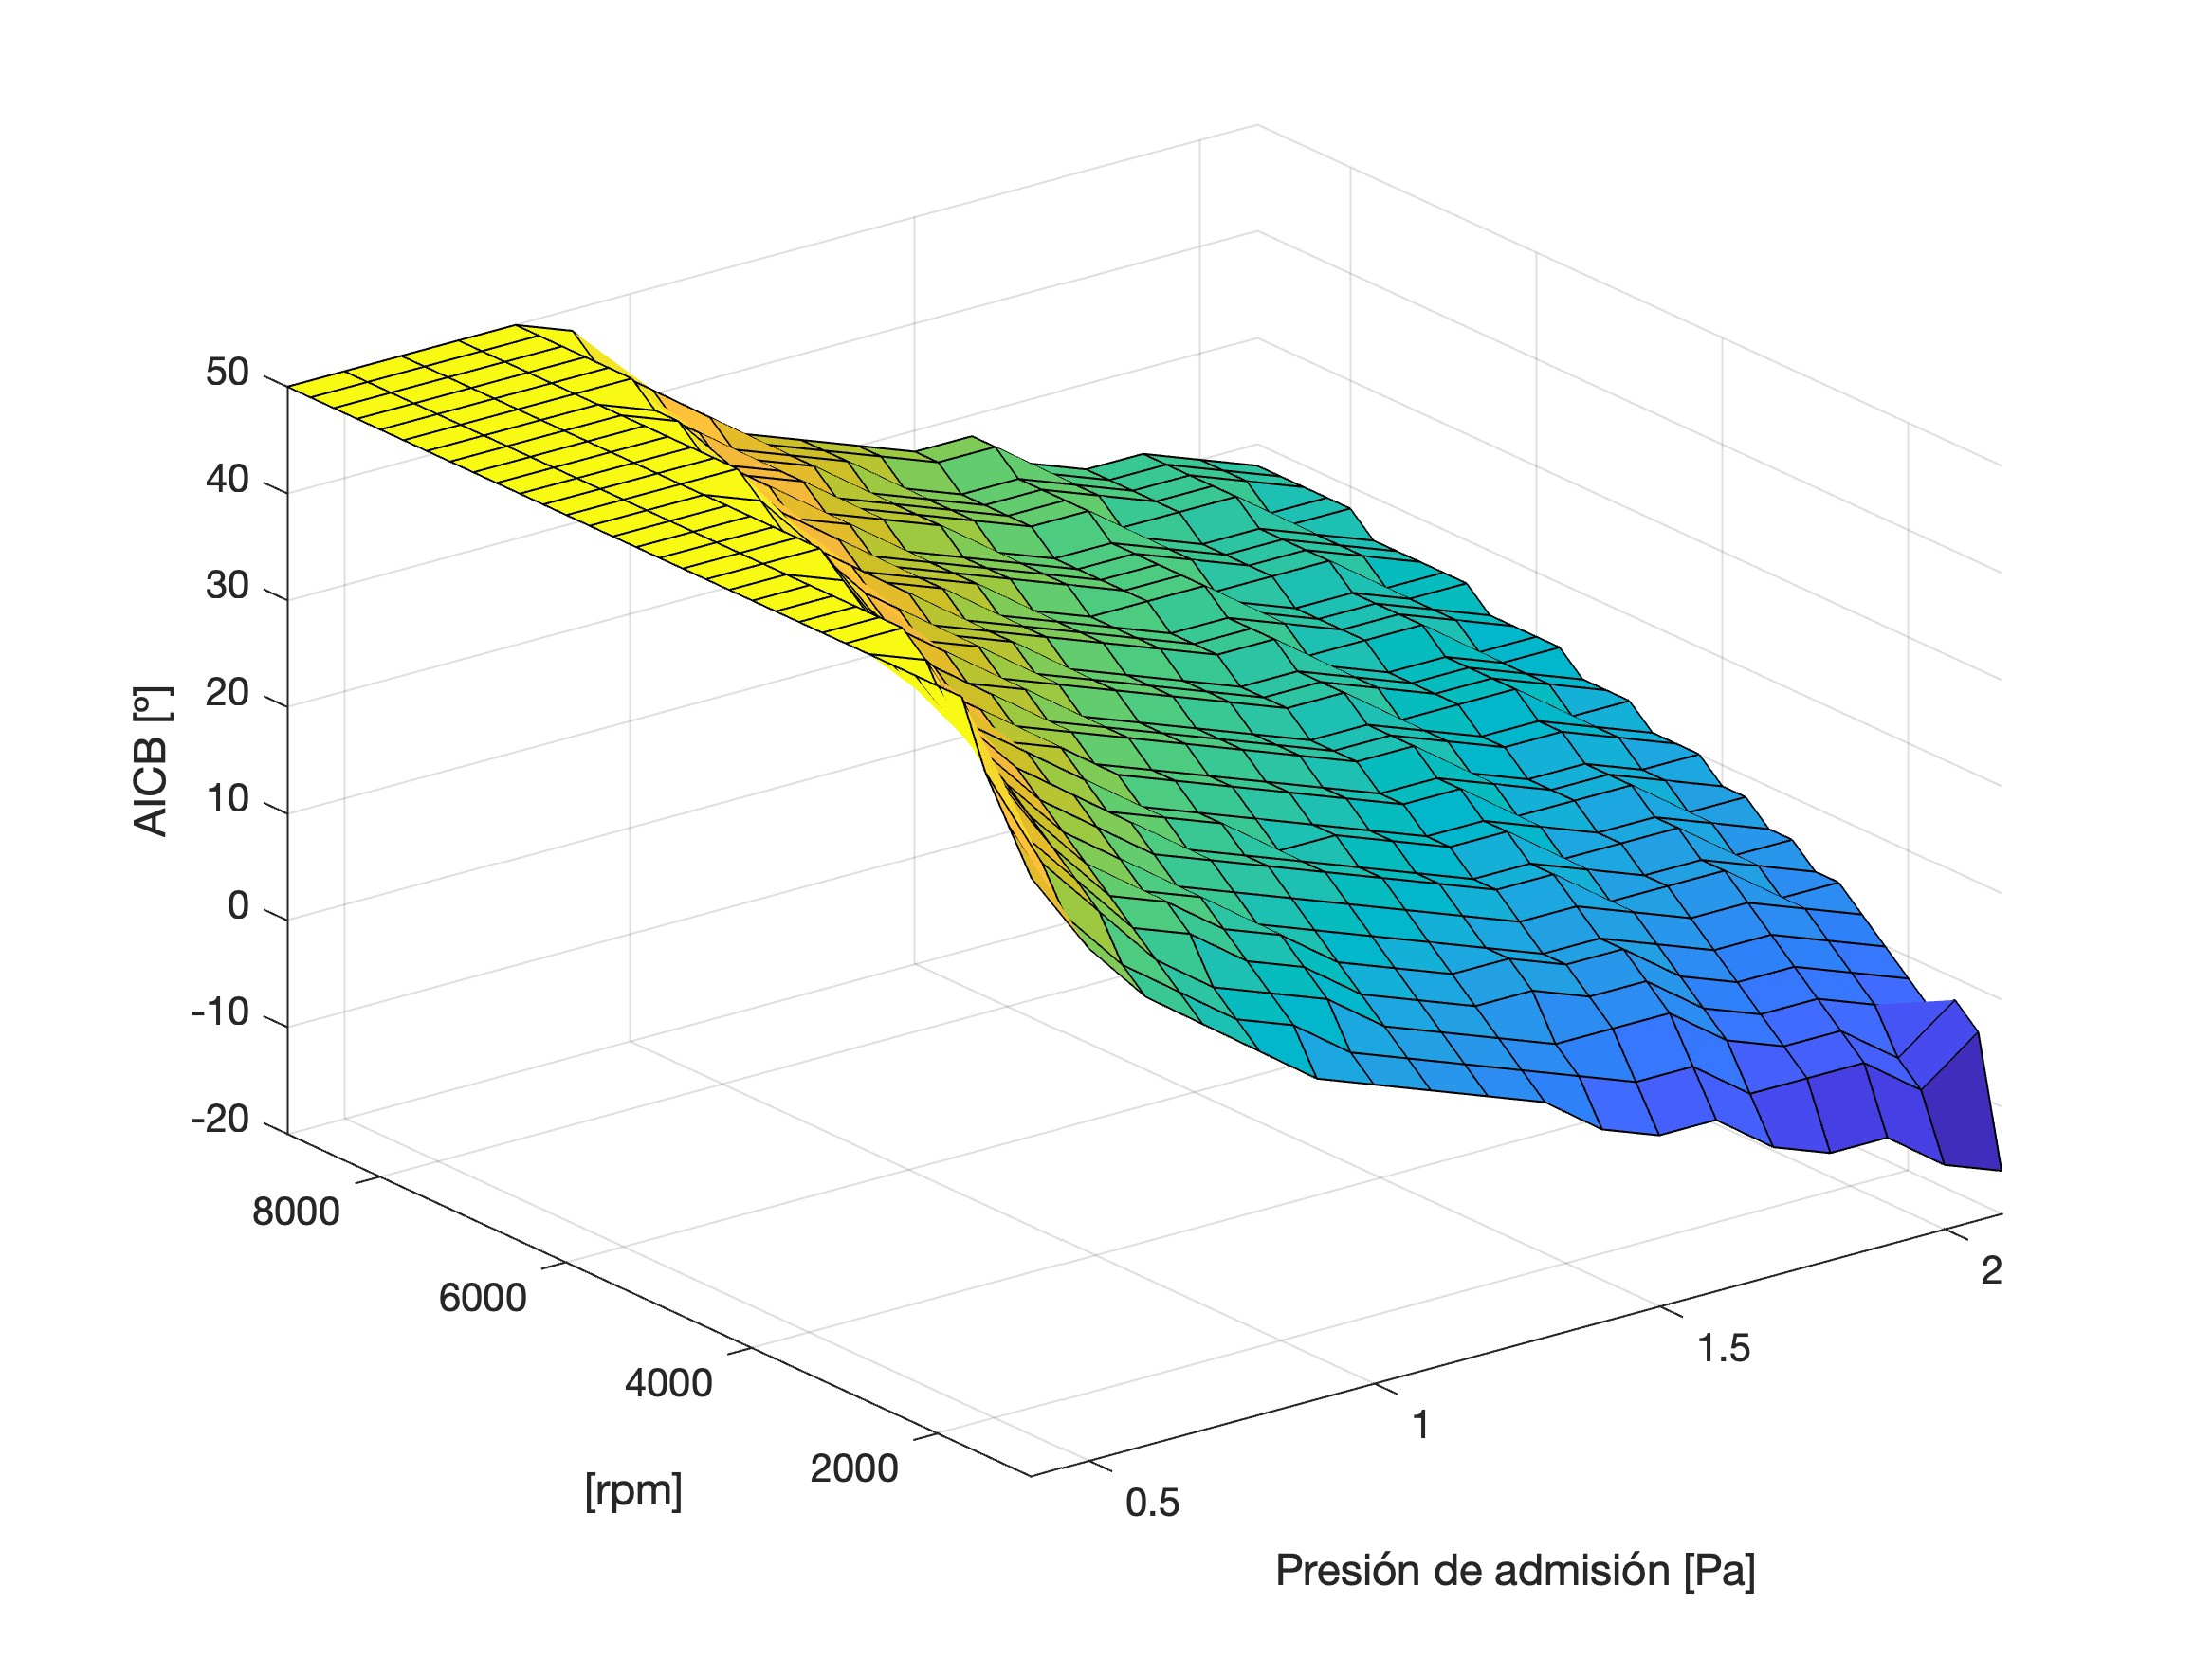
\includegraphics[width=0.6\linewidth]{Figures/01/ignitionmap.jpg}
    \caption{Mapa de ignición del motor finalizado.}
    \label{fig:mapa_completo}
\end{figure}

\section{Optimización por métodos numéricos} \label{s:section_08}

Por último se ha hecho uso de algoritmos de optimización para comparar los valores de los ángulos de adelanto de combustión, retardo al cierre de admisión y %
adelanto a la apertura de escape obtenidos de forma cualitativa para maximizar la potencia con los obtenidos al resolver el problema de optimización. %
Por el funcionamiento interno del código los valores del RCA, AAE y AICB son tratados como números enteros, por esta razón un método gradiente no resultaría %
práctico y se ha hecho uso de algoritmos genéticos. La optimización se ha realizado tomando como variables de diseño los tres ángulos mencionados y como función objetivo %
la potencia del ciclo sin alterar el resto de parámetros y con la restriccion de que no se llegue a detonación.
Los resultados obtenidos mediante la función \textit{ga} del \textit{Optimization Toolbox} de MATLAB se muestran a continuación:

\begin{figure}[H]
    \centering
    \begin{subfigure}[b]{0.45\textwidth}
        \centering
        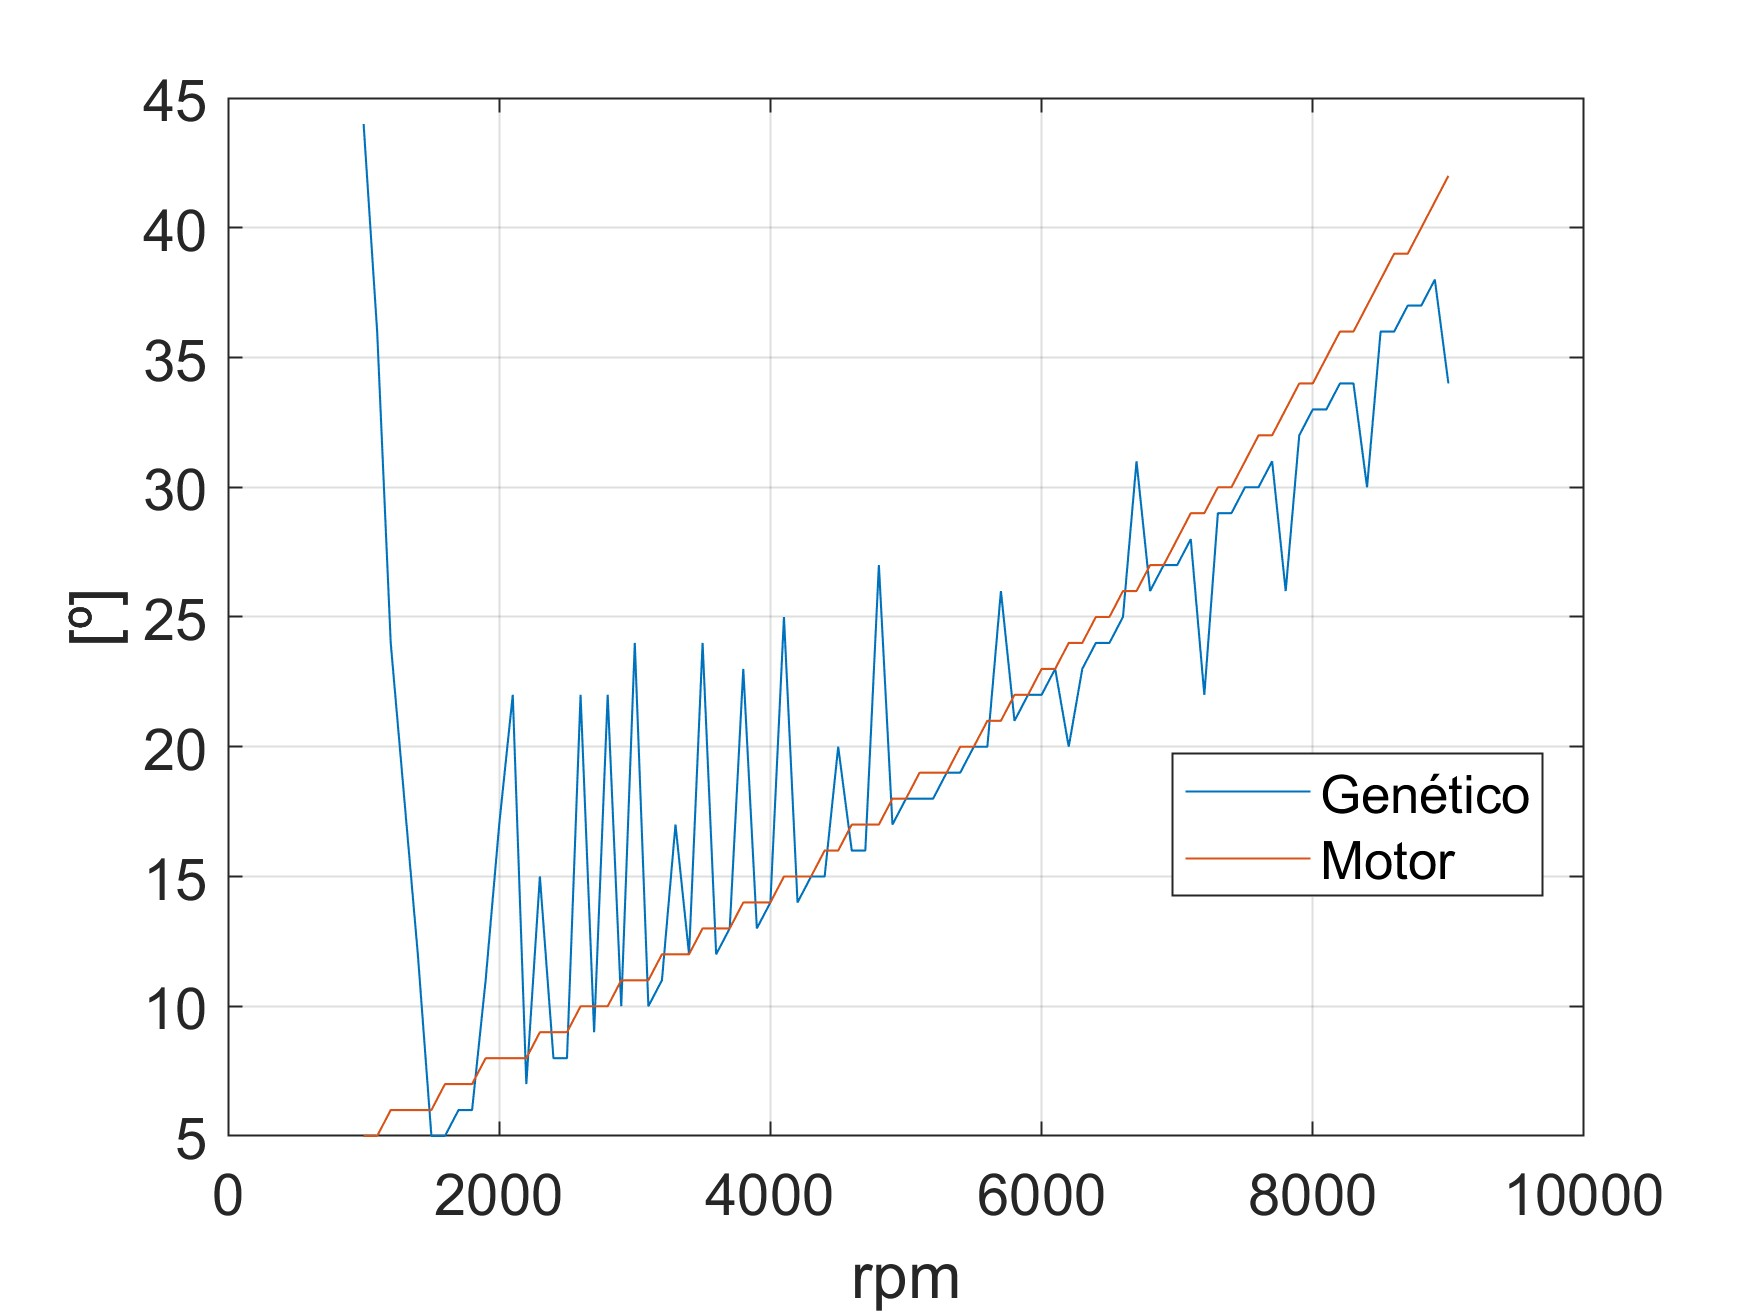
\includegraphics[width=\linewidth]{Figures/01/opti_RCA.jpg}
        \caption{Retardo del cierre admisión.}
        \label{fig:opti_RCA}
    \end{subfigure}
    \hfill
    \begin{subfigure}[b]{0.45\textwidth}
        \centering
        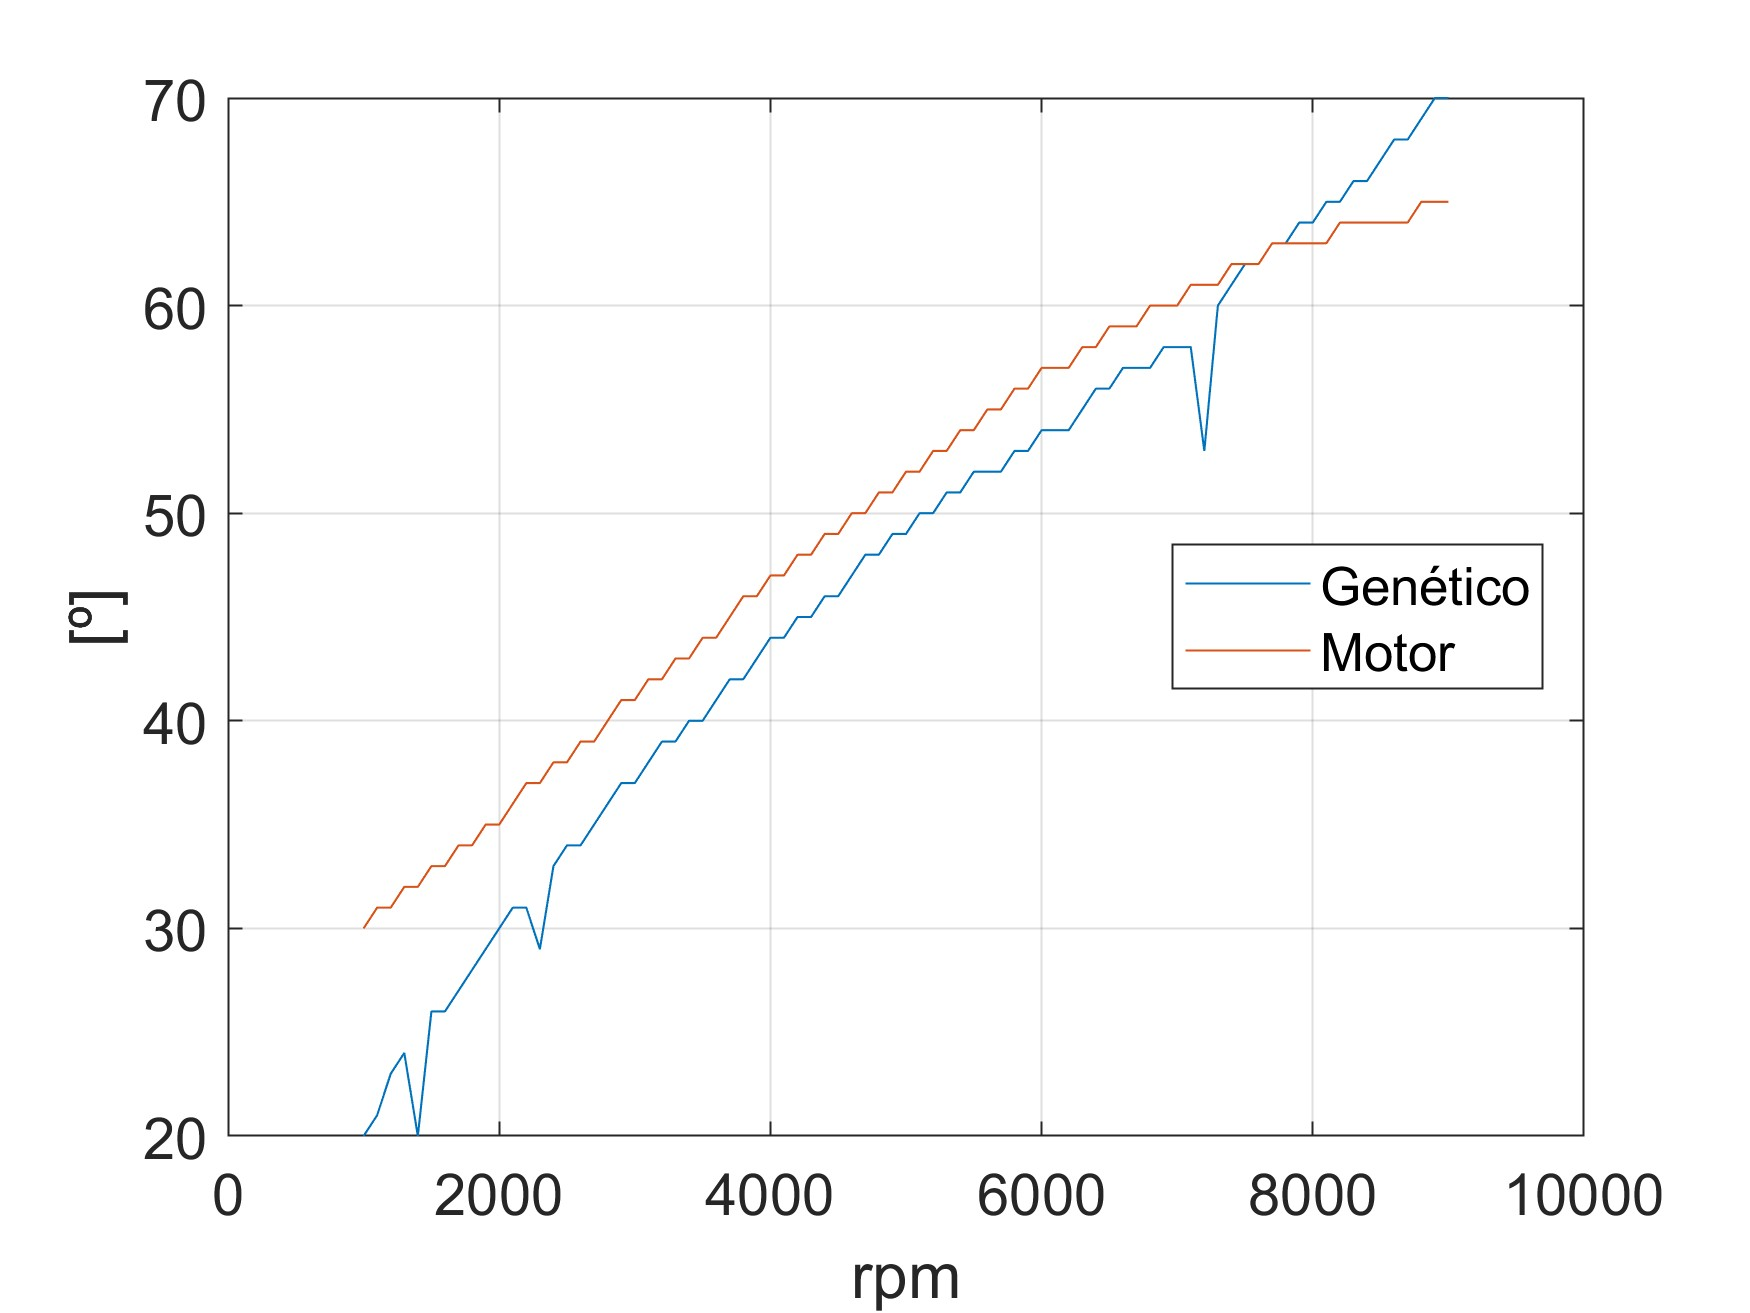
\includegraphics[width=\linewidth]{Figures/01/opti_AAE.jpg}
        \caption{Adelanato a la apertura de escape.}
        \label{fig:opti_AAE}
    \end{subfigure}
    \\
    \begin{subfigure}[b]{0.45\textwidth}
        \centering
        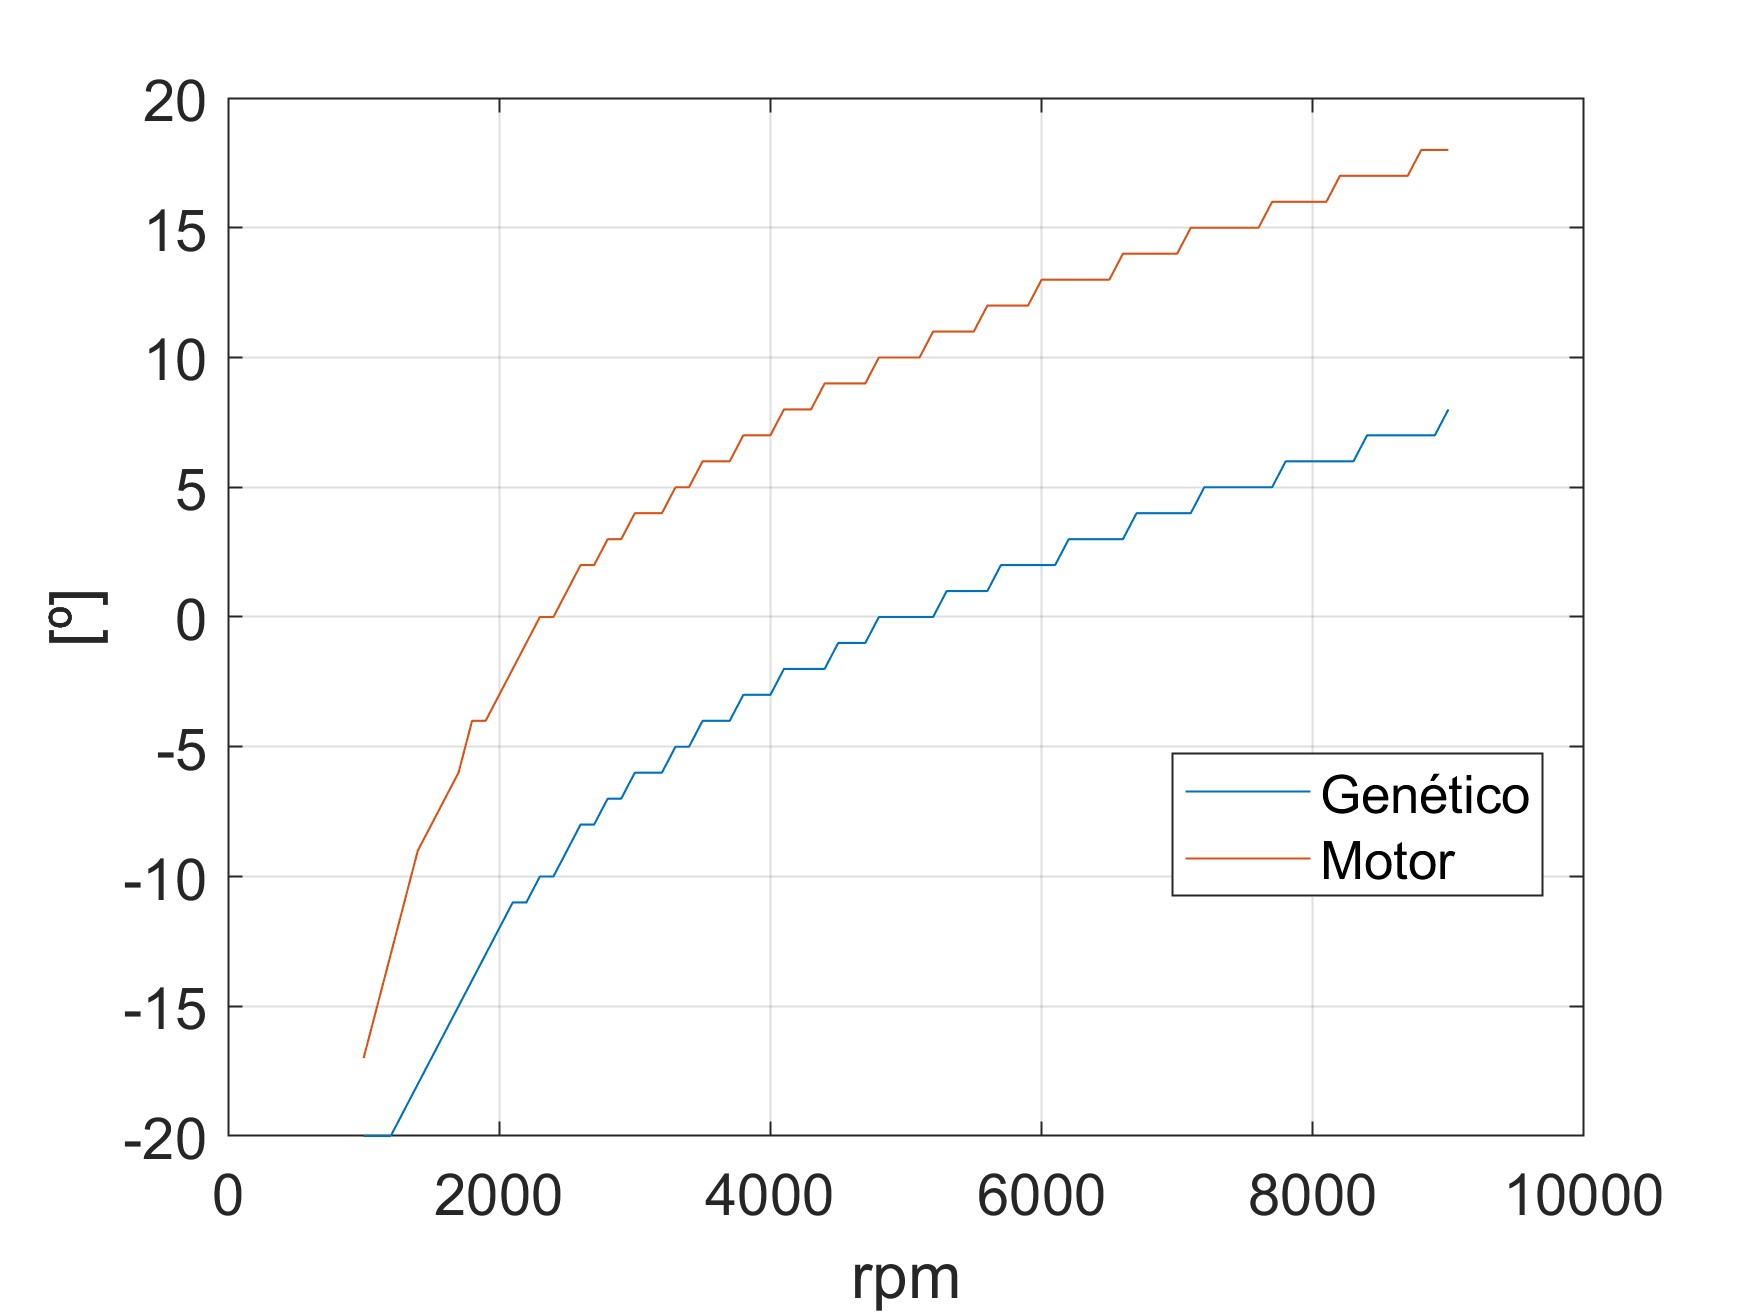
\includegraphics[width=\linewidth]{Figures/01/opti_AICB.jpg}
        \caption{Adelanto al inicio de combustión.}
        \label{fig:opti_AICB}
    \end{subfigure}
    \caption{Ángulos óptimos obtenidos de forma cualitativa y mediante el algoritmo genético en función de las rpm.}
    \label{fig:opti_angles}
\end{figure}


\begin{figure}[H]
    \centering
    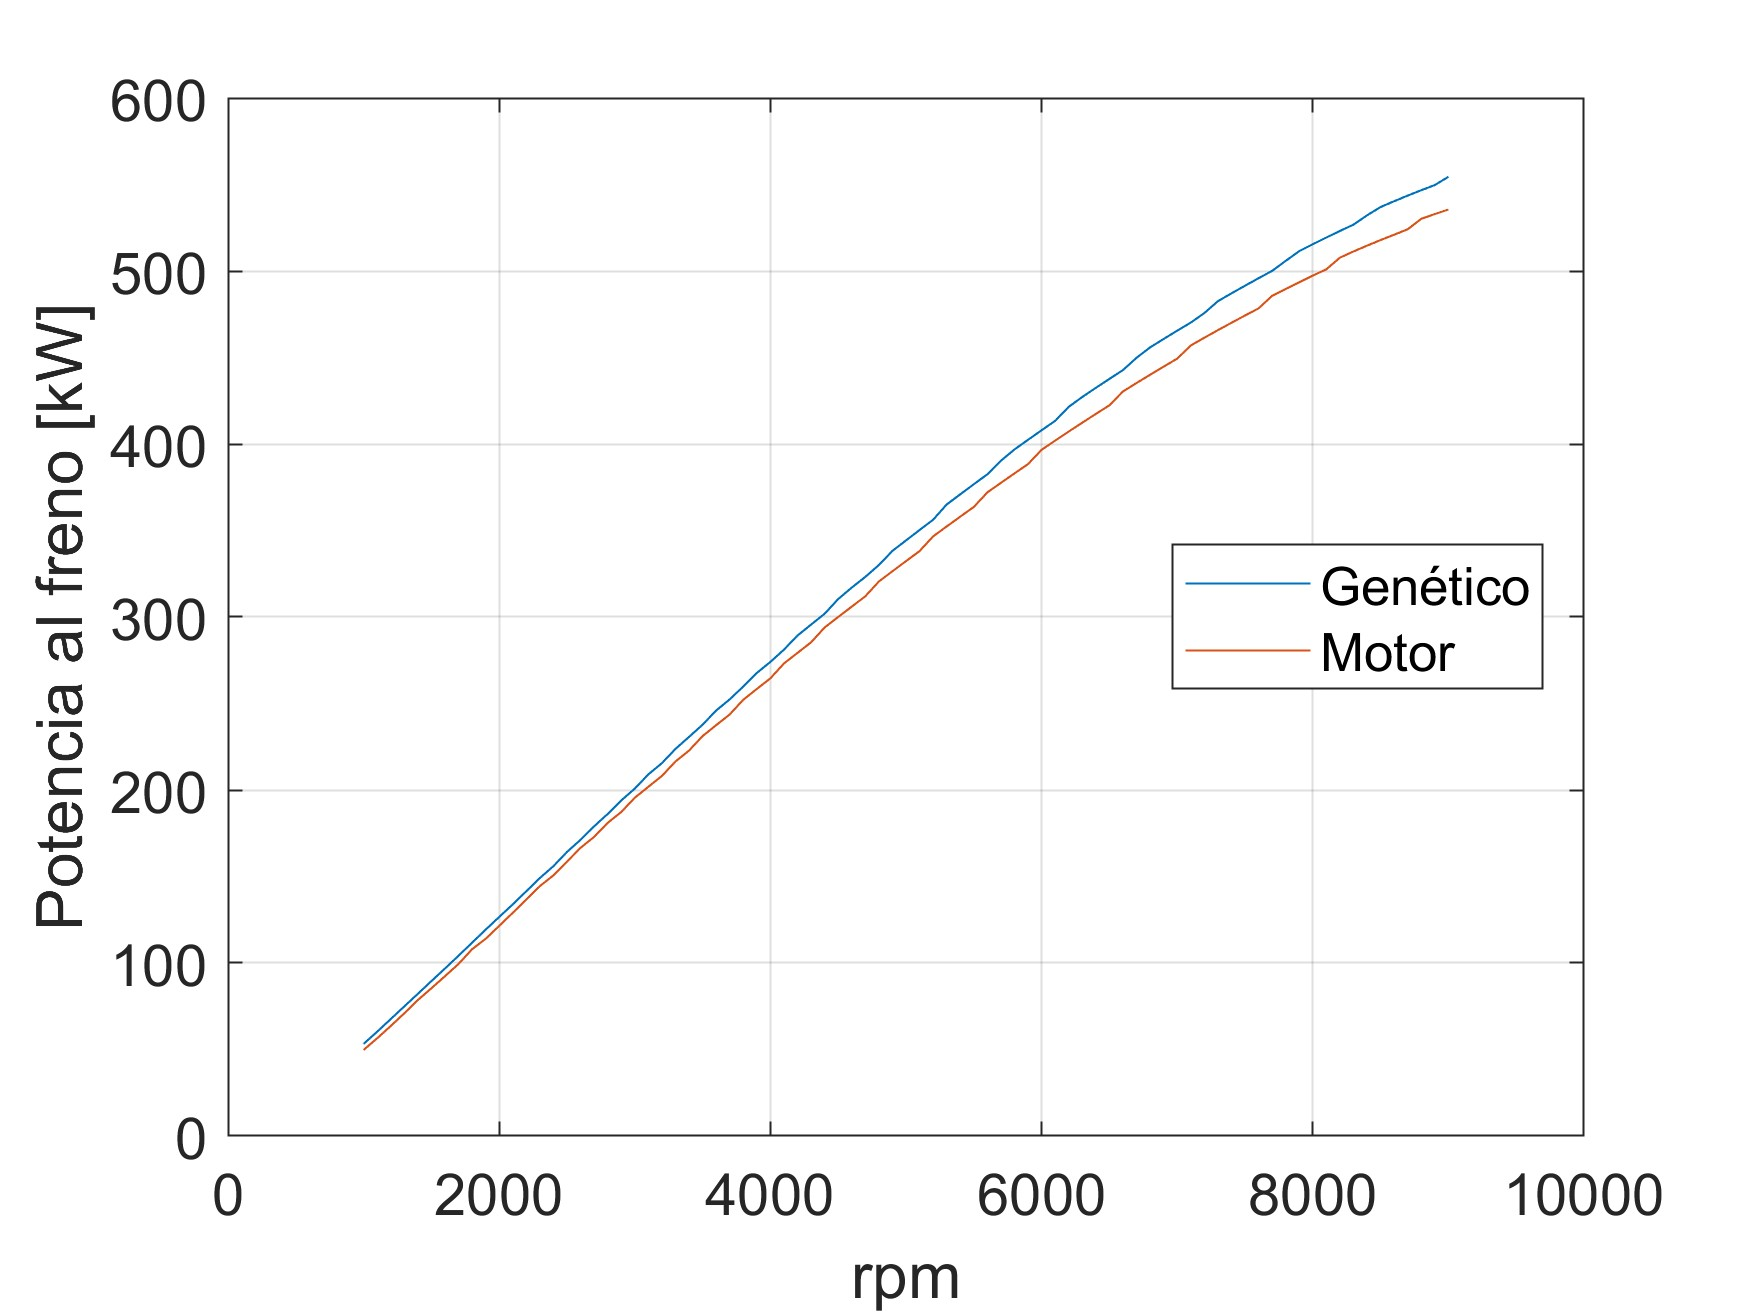
\includegraphics[width=0.6\linewidth]{Figures/01/opti_pot.jpg}
    \caption{Potencia al freno del motor usado y el optimizado frente a rpm.}
    \label{fig:opti_pot}
\end{figure}

\begin{figure}[H]
    \centering
    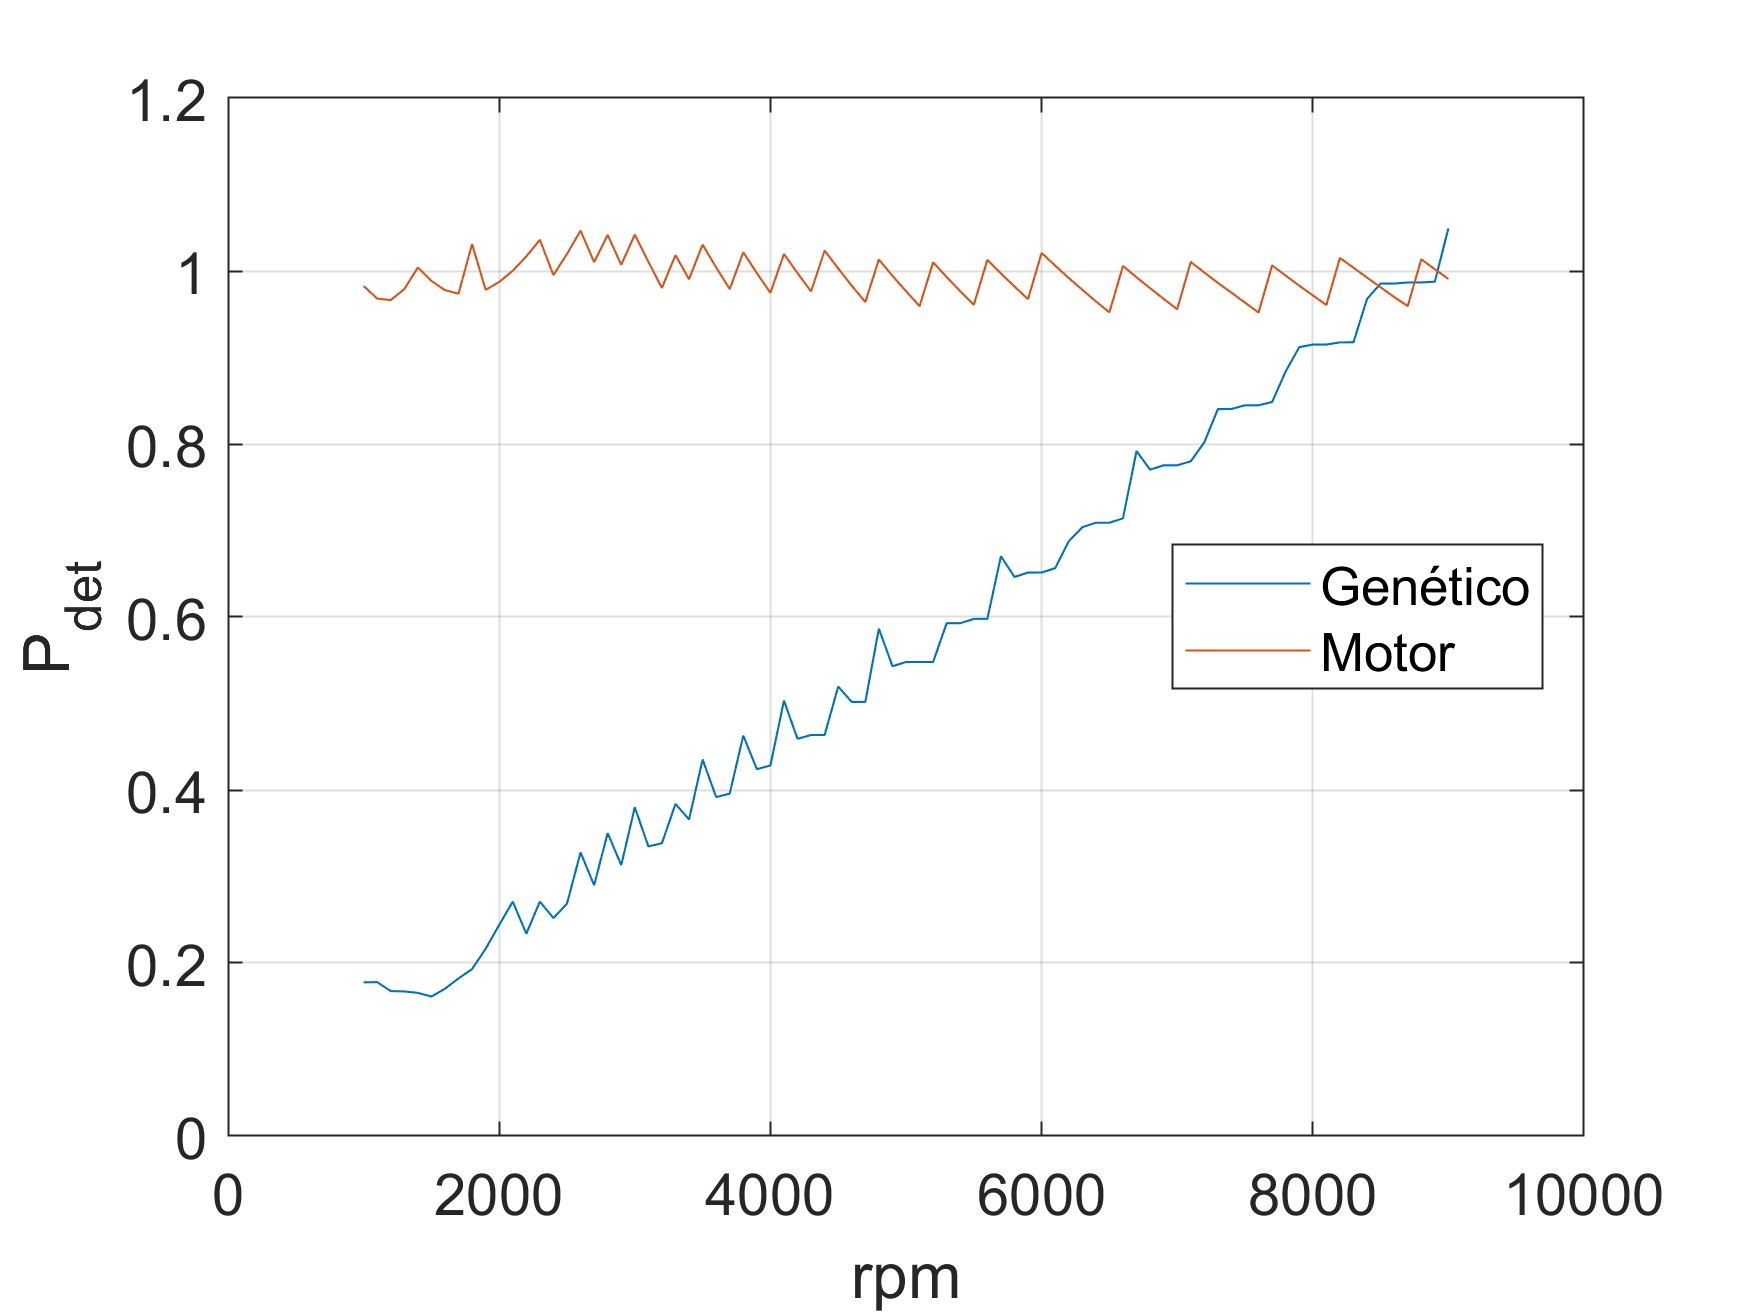
\includegraphics[width=0.6\linewidth]{Figures/01/opti_pdet.jpg}
    \caption{Peligro de detonación del motor usado y el optimizado frente a rpm.}
    \label{fig:opti_pdet}
\end{figure}

A la vista de las figuras \ref{fig:opti_angles} se comprueba que las tendencias obtenidas de forma cualitativa coinciden con las obtenidas con la optimización. A bajas rpm se observa %
cierta falta de consistencia en los valores óptimos del RCA, figura \ref{fig:opti_RCA}, esto se puede deber a la inestabilidad propia de los métodos genéticos. La mayor diferencia se %
observa el AICB que es entre $5-10^\circ$ inferior al usado, figura \ref{fig:opti_AICB}. Sin  embargo, se observa que se ha obtenido un incremento de potencia marginal frente al obtenido mediante el análisis cualitativo, figura \ref{fig:opti_pot} %
mostrando la fidelidad de este método que tan solo requiere del ánalisis de gráficas y datos obtenidos directamente frente a las varias horas de cálculo que requiere el algoritmo de optimización %
para obtener resultados que como se puede ver no son totalmente precisos. La otra diferencia más destacable es que mientras en el motor usado siempre se está operando en condiciones próximas a la %
detonación en el obtenido por optimización solo se llega a esta situación a altas rpm, figura \ref{fig:opti_pdet}.


\section{Conclusiones} \label{s:section_09}

A lo largo del desarrollo de este trabajo e informe, se ha aprendido el proceso para prediseñar y dimensionar un motor (si bien con un objetivo ciertamente arbitrario). Los alumnos autores de este informe dejan pendiente el aprender la utilización de software algo más especializado y, en especial, de un modelo más correcto de turboalimentación/sobrealimentación del motor, pues la mayor parte de motores actuales se encuentran configurados de tal manera.

En cuanto al motor específico diseñado a lo largo de este trabajo, es interesante observar que se han conseguido números de potencia bastante superiores a los desarrollados por el coche real en el que se ha inspirado el motor. Dichas discrepancias provienen de que para el motor estudiado no se ha tenido en cuenta la durabilidad del mismo (se podría mejorar disminuyendo el área de las válvulas, la presión de soplado del turbo...).

